\chapter{Zusammenspiel der sprachlichen Markierungen}\label{zusammenspiel}
 %\noindent
In diesem Kapitel werden alle erhobenen Phänomene in ihrer Summe, ihrer räumlichen und systematischen Verteilung, zusammengetragen. Die erhobenen Daten können aus zwei Perspektiven betrachtet werden: Zum einen kann die Perspektive auf die Verteilung der Phänomene (Kapitel \ref{clusterPhänomene}, S.\, \pageref{clusterPhänomene}) gerichtet sein, zum anderen auf die Ähnlichkeit/Unähnlichkeit der Quellen (Kapitel \ref{clusterQuellen}, S.\, \pageref{clusterQuellen}). 

Eine wichtige Methode ist hier die hierarchische Clusteranalyse. In einer Clusteranalyse wird berechnet, ob und welche Phänomene gemeinsam auftreten. Die Berechnung eines hierarchischen Ward-Clusters erfolgt über die Quadrierung der euklidischen Distanz zwischen zwei Messwerten, und zwar nach der Formel:\footnote{Verwendeter \hai{R}-Code für die nachfolgenden Clusteranalysen: {\ttfamily \scriptsize{d <- dist(DATEINAME, method = \grqq euclidean\grqq) (für Distanzmatrix) 
fit <- hclust(d, method=\grqq ward.D2\grqq)
 plot(fit) (zeichnet das Dendrogramm)
groups <- cutree(fit, k=5) (teilt den Baum in 5 Cluster) 
rect.hclust(fit, k=5, border="red") (zeichnet rote Quadrate um die 5 Cluster)}}}

\begin{center}\begin{math}
d\textsubscript{ij} = d(\{X\textsubscript{i}\}, \{X\textsubscript{j}\}) = |X\textsubscript{i} – X\textsubscript{j} |^2 
\end{math}
\end{center} 
\vspace{0.2cm}

Das Ergebnis einer Clusteranalyse wird üblicher Weise in Dendrogrammen graphisch dargestellt. Dieses \textit{Baumschema} veranschaulicht, welche Datensätze nah (wenige Knoten zwischen zwei Datenpunkten) bzw. fern (viele Knoten zwischen zwei Datenpunkten) zueinander liegen, d.\,h. sich ähnlich/unähnlich zueinander verhalten.

Da zwei Quellen (\hai{NF} Hamburg, 1749 u. \hai{PS} Berlin, 1808) nur sehr geringe \hai{{\LiJi}}-Evidenz liefern und die vorhandenen Daten der beiden Texte nur periphere, im Gesamtbild des \hai{{\LiJi}} selten auftretende Phänomene darstellen, fallen diese beiden Quellen in der Darstellung des Zusammenspiels der sprachlichen Markierungen nicht ins Gewicht und sie bilden eine eigene Gruppe. Insgesamt verringert sich damit an dieser Stelle das \isi{Korpus} zum \hai{chrLiJi1} von 53 Texten auf 51 Texte.

Eine exakte Differenzierung zwischen Phänomenen, die dem \hai{{\WJ}} und/oder \hai{{\OJ}} entsprechen bzw. nicht entsprechen, kann dabei allerdings nicht vorgenommen werden. Wie in den Einzelananlysen dargestellt, ist eine solche Entscheidung in den meisten Fällen nicht leicht zu treffen. Die nachfolgende Zusammenschau zeigt also nur rein quantitative Werte sprachlicher Manipulationsstrategien des \hai{{\LiJi}}, nicht aber deren qualitative Distribution. Die Datengrundlage für die nachfolgenden Darstellungen und Berechnungen der Zusammenschau literaturjiddischer Manipulationen im \hai{chrLiJi1} liegt im Anhang \ref{appendixphaenall} (S.\, \pageref{appendixphaenall}) tabellarisch vor.

 
\section{Distribution der Phänomene untereinander}\label{clusterPhänomene}
 %\noindent
Die folgenden Darstellungen beruhen auf der Belegsumme von 58 beschriebenen Einzelphänomenen der drei grammatischen Ebenen (Phonologie, \isi{Morphologie} und \isi{Syntax}). Ein Phänomen tritt im Durchschnitt in 12 (von 51) Quellen auf.  Die Standardabweichung von 10 zeigt an, dass eine große Streuung innerhalb der Quellen vorliegt, was die Anzahl der verwendeten Phänomene betrifft. 

Richten wir zunächst unseren Blick auf die zeitliche Verteilung der Phänomene in ihrer Summe. Wie das Diagramm in Abbildung \ref{boxplotjahrsumme} zeigt, findet sich besonders zwischen den 1770ern und 1870ern, also dem zentralen Zeitraum unseres Samples, eine besonders große Streuung bezüglich der Anzahl der zum Einsatz kommenden Phänomene. Die wenigen Quellen im \isi{Korpus} des frühen 18. Jahrhunderts zeigen eine vergleichsweise geringe Gesamtzahl an Phänomenen.  Quellen des frühen 20. Jahrhunderts hingegen weisen überdurchschnittlich viele Phänomene in den einzelnen Quellen auf. Trotz hoher Streuung lässt sich somit ein Anstieg an Phänomenen vom 18. zum 20. Jahrhundert feststellen, der jedoch ab der Mitte des 19. Jahrhunderts nachlässt.



\begin{figure}
\centering
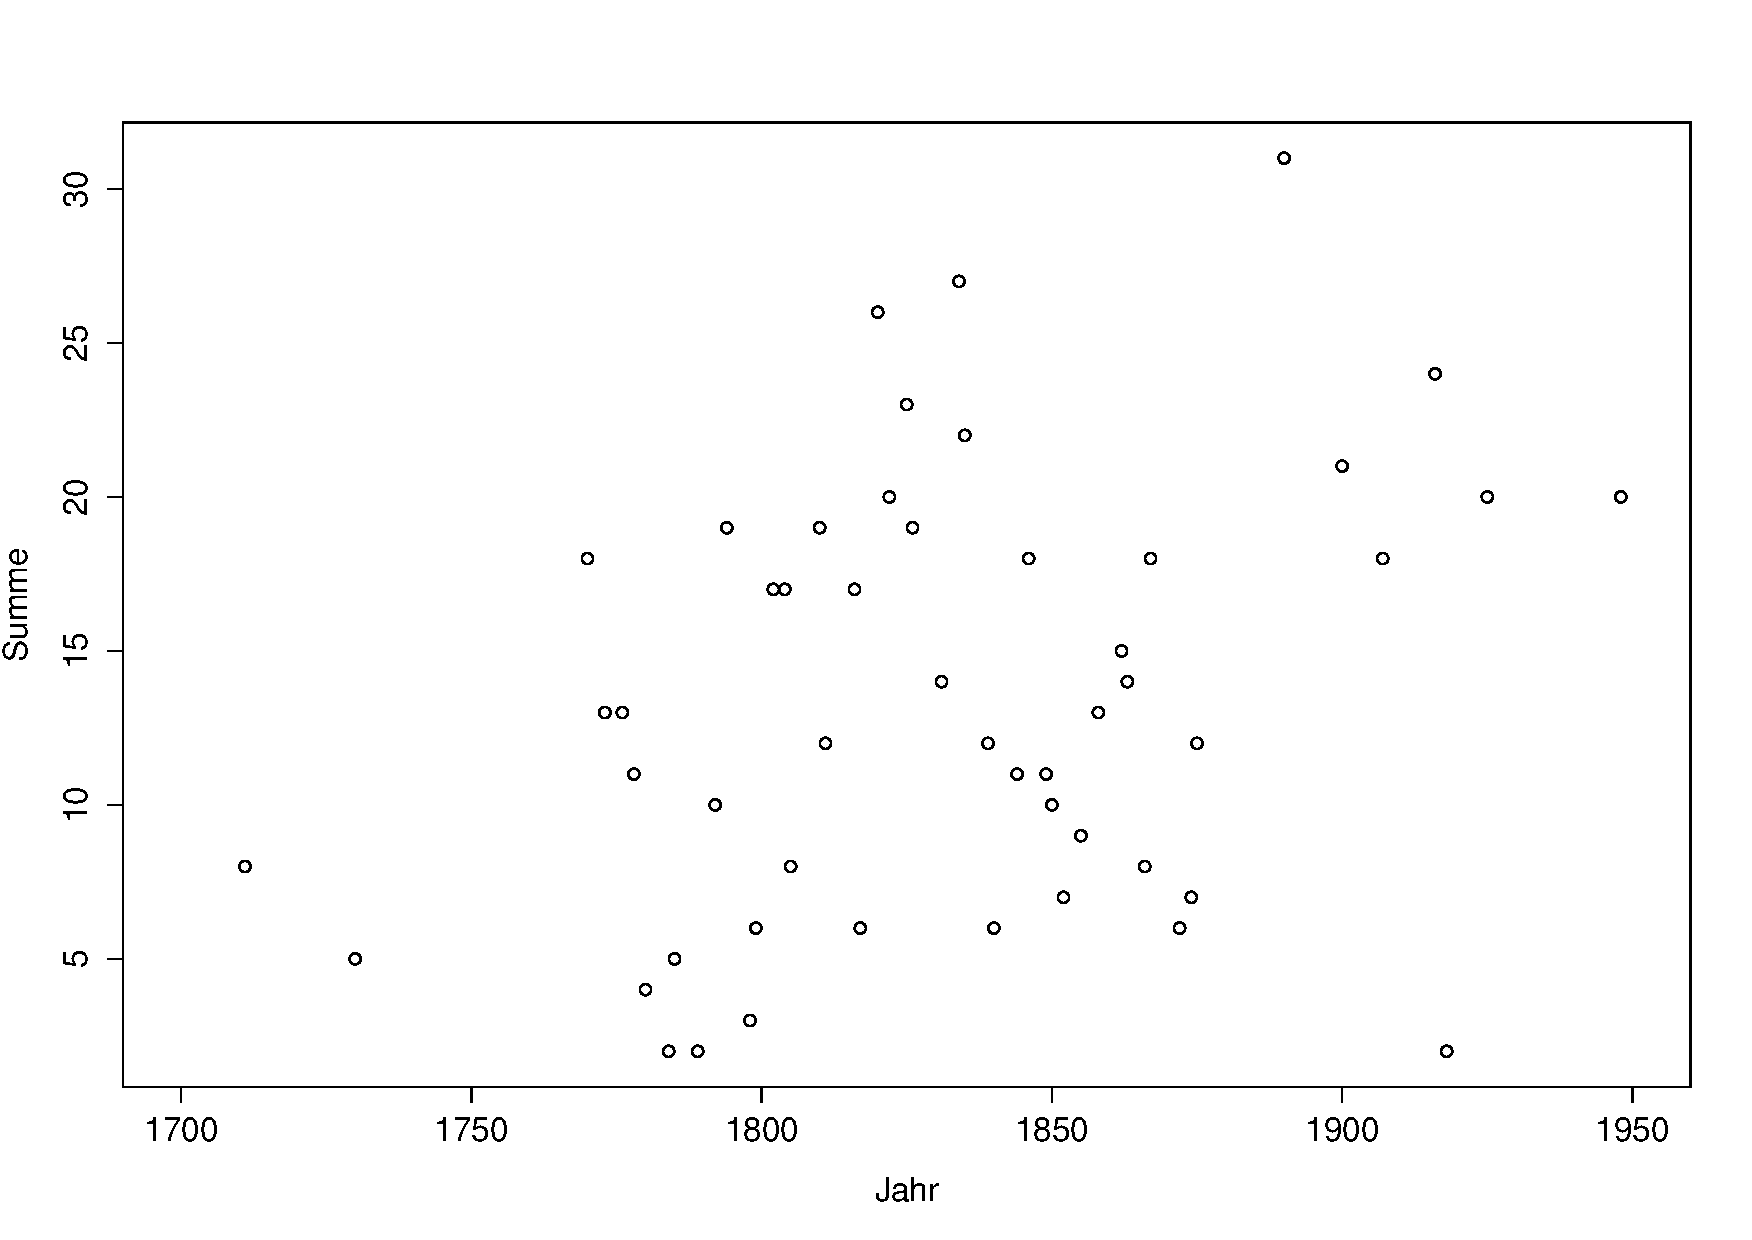
\includegraphics[width=\textwidth]{figures/Rplot_Summe_hai.pdf}
		\caption{\label{boxplotjahrsumme}Summe der Phänomene im \hai{chrLiJi1}}
	\end{figure}
 


 \begin{figure}
 \farbgrafik
\resizebox{.9\textwidth}{!}{
	\begin{tikzpicture}
		\begin{axis}[only marks, 
 width=0.82\textwidth,height=\textheight,
		legend style={at={(1,1)},xshift=+0.2cm,%yshift=0.02cm,
		anchor=north west,nodes=left, font=\tiny,row sep=-0.06ex},
			%title={Funktionstypen des sp\"aten Westjiddisch},
			xtick={1700, 1725, 1750, 1775, 1800, 1825, 1850, 1875, 1900, 1925, 1950, 1975}, ytick=\empty,
			x tick label style={/pgf/number format/1000 sep=}, 
			y tick label style={/pgf/number format/1000 sep=},
			extra y tick style={grid=major,
				tick label style={, ,}},
			        ymin=0.51,
				ymax=58.9,
				y=3.35mm,
			ylabel={Phänomene},
			enlarge x limits=0.03]	

\addplot [mark=square*, Goldenrod] table [x=jahr, y=NP] {figures/EX_NP_58.txt};\addlegendentry{\hai{{\NP}}-Ex}
\addplot [mark=square*, blue] table [x=jahr, y=PP] {figures/EX_PP_57.txt};\addlegendentry{\hai{{\PP}}-Ex}
\addplot [mark=square*, orange] table [x=jahr, y=AP] {figures/EX_AP_56.txt};\addlegendentry{\hai{{\AP}}-Ex}
 \addplot [mark=square*, red] table [x=jahr, y=ADV] {figures/EX_ADV_55.txt};\addlegendentry{ \hai{ADV}-Ex}
\addplot [mark=square*, SkyBlue] table [x=jahr, y=V2_weil] {figures/all_V2_weil_54.txt};\addlegendentry{ \textit{weil}-\hai{V2}}
\addplot [mark=square*, WildStrawberry] table [x=jahr, y=V2_dass] {figures/all_V2_dass_53.txt};\addlegendentry{\textit{dass}-\hai{V2}}
\addplot [mark=square*, BlueViolet] table [x=jahr, y=particl] {figures/all_particl_52.txt};\addlegendentry{ rechtsadjzt. Verbpartikel}
 \addplot [mark=square*, RedOrange] table [x=jahr, y=VPR] {figures/all_VPR_51.txt};\addlegendentry{\hai{{\VPR}}}
\addplot [mark=square*, OliveGreen] table [x=jahr, y=was_SU] {figures/all_was_SU_50.txt};\addlegendentry{\textit{was} Relativpartikel}
\addplot [mark=square*, Goldenrod] table [x=jahr, y=SU_WO] {figures/all_SU_WO_49.txt};\addlegendentry{ \textit{wo} Relativpartikel}
\addplot [mark=square*, teal] table [x=jahr, y=VR] {figures/all_VR_48.txt};\addlegendentry{\hai{{\VR}}}
\addplot [mark=square*, black] table [x=jahr, y=123VR] {figures/all_123VR_47.txt};\addlegendentry{1-2-3 Verbcluster}
\addplot [mark=square*, green] table [x=jahr, y=NOIPP] {figures/all_noIPP_46.txt};\addlegendentry{\hai{no-IPP}}
 \addplot [mark=square*, gray] table [x=jahr, y=Ndnegation] {figures/all_negation_45.txt};\addlegendentry{negative doubling}
\addplot [mark=square*, Thistle] table [x=jahr, y=kommenzugehen] {figures/all_kommenzugehen_44.txt};\addlegendentry{\textit{kommen-zu}-Konstr.}

\addplot [very thick, mark=triangle*,  BrickRed] table [x=jahr, y=sein] {figures/all_sein_43.txt};\addlegendentry{\textit{sein}}
\addplot [very thick, mark=triangle*, WildStrawberry] table [x=jahr, y=Pluralsuffix] {figures/all_Pluralsuffix_42.txt};\addlegendentry{Pluralsuffixe}
\addplot [very thick, mark=triangle*, teal] table [x=jahr, y=PronomenHOEF_DAT] {figures/all_PronomenHOEF_DAT_41.txt};\addlegendentry{{\Pron} Höfl.{Dat}}
\addplot [very thick, mark=triangle*, black] table [x=jahr, y=PronomenHOEF_NOM] {figures/all_PronomenHOEF_NOM_40.txt};\addlegendentry{{\Pron} Höfl.{\Nom}}
\addplot [very thick, mark=triangle*, green] table [x=jahr, y=Pronomen1PLNOM_1SGDAT] {figures/all_Pronomen1PLNOM_1SGDAT_39.txt};\addlegendentry{{\Pron} 1.{\Pl}{\Nom}=1.{\Sg}{Dat}}
\addplot [very thick, mark=triangle*, gray] table [x=jahr, y=Pronomen3SG_AKK] {figures/all_Pronomen3SG_AKK_38.txt};\addlegendentry{{\Pron} 3.{\Sg}{\Akk}}
 \addplot [very thick, mark=triangle*, Thistle] table [x=jahr, y=Pronomen2SG_DAT] {figures/all_Pronomen2SG_DAT_37.txt};\addlegendentry{{\Pron} 2.{\Sg}{Dat}}
\addplot [very thick, mark=triangle*, Melon] table [x=jahr, y=Pronomen1SG_AKK] {figures/all_Pronomen1SG_AKK_36.txt};\addlegendentry{{\Pron} 1.{\Sg}{\Akk}}
\addplot [very thick, mark=triangle*, CornflowerBlue] table [x=jahr, y=Pronomen1SG_DAT] {figures/all_Pronomen35SG_DAT_35.txt};\addlegendentry{{\Pron} 1.{\Sg}{Dat}}
\addplot [very thick, mark=triangle*, magenta] table [x=jahr, y=KasusPraepPL_DAT] {figures/all_KasusPraepPL_DAT_34.txt};\addlegendentry{Kasus (\hai{{\PP}}) {\Pl}{Dat}}
\addplot [very thick, mark=triangle*, ForestGreen] table [x=jahr, y=KasusPraepPL_AKK
] {figures/all_KasusPraepPL_AKK_33.txt};\addlegendentry{Kasus (\hai{{\PP}}) {\Pl} {\Akk}}
\addplot [very thick, mark=triangle*, Dandelion] table [x=jahr, y=KasusPraepDAT_statt_AKK
] {figures/all_PraepDAT_statt_AKK_32.txt};\addlegendentry{Kasus (\hai{{\PP}}) {\Sg}{Dat}}
\addplot [very thick, mark=triangle*, SkyBlue] table [x=jahr, y=KasusPraepAKK_statt_DAT] {figures/all_PraepAKK_statt_DAT_31.txt};\addlegendentry{Kasus (\hai{{\PP}}) {\Sg} {\Akk}}
\addplot [very thick, mark=triangle*, YellowGreen] table [x=jahr, y=KasusnvolleNPPL_NOM] {figures/all_KasusnvolleNPPL_NOM_30.txt};\addlegendentry{Kasus (\hai{{\NP}}) {\Pl}{\Nom}}
\addplot [very thick, mark=triangle*, RoyalPurple] table [x=jahr, y=KasusnvolleNPSG_M_DAT] {figures/all_KasusnvolleNPSG_M_DAT_29.txt};\addlegendentry{Kasus (\hai{{\NP}}) {\Sg}{\mask}{Dat}}
\addplot [very thick, mark=triangle*, orange] table [x=jahr, y=KasusnvolleNPSG_M_NOM] {figures/all_KasusnvolleNPSG_M_NOM_28.txt};\addlegendentry{Kasus (\hai{{\NP}}) {\Sg}{\mask}{\Nom}}
\addplot [very thick, mark=triangle*, Maroon] table [x=jahr, y=OJ_GENUS] {figures/all_OJGenus_27.txt};\addlegendentry{oj. Genus}
\addplot [very thick, mark=triangle*, Goldenrod] table [x=jahr, y=gePartizip] {figures/all_gePart_26.txt};\addlegendentry{ \textit{ge-}Partizip}
\addplot [very thick, mark=triangle*, LimeGreen] table [x=jahr, y=lichPL] {figures/all_lichPL_25.txt};\addlegendentry{\textit{-lich} {\Pl} {\Dim}}

\addplot [mark=*, Fuchsia] table [x=jahr, y=wb] {figures/all_wb_24.txt};\addlegendentry{<w> statt <b>}
\addplot [mark=*, BrickRed] table [x=jahr, y=LVp] {figures/all_LVp_23.txt};\addlegendentry{germ. -\textit{pp}-}
\addplot [mark=*, MidnightBlue] table [x=jahr, y=kg] {figures/all_kg_22.txt};\addlegendentry{<k> statt <g>}
\addplot [mark=*, black] table [x=jahr, y=bp] {figures/all_bp_21.txt};\addlegendentry{<b> statt <p>}
\addplot [mark=*, Thistle] table [x=jahr, y=pb] {figures/all_pb_20.txt};\addlegendentry{<p> statt <b>}
 \addplot [mark=*, LimeGreen] table [x=jahr, y=td] {figures/all_td_19.txt};\addlegendentry{<t> statt <d>}
\addplot [mark=*, ProcessBlue] table [x=jahr, y=dt] {figures/all_dt_18.txt};\addlegendentry{<d> statt <t>}
\addplot [mark=*, Maroon] table [x=jahr, y=s] {figures/all_s_z_17.txt};\addlegendentry{<s> statt <z>}
\addplot [mark=*, Melon] table [x=jahr, y=sz] {figures/all_sz_z_16.txt};\addlegendentry{<ß> statt <z>}
 \addplot [mark=*, RoyalPurple] table [x=jahr, y=scht_anlaut] {figures/all_scht_an_15.txt};\addlegendentry{<scht> (\isi{Anlaut})}
\addplot [mark=*, YellowGreen] table [x=jahr, y=scht_auslaut] {figures/all_scht_aus_14.txt};\addlegendentry{<scht> (\isi{Auslaut})}
\addplot [mark=*, CarnationPink] table [x=jahr, y=oe_i] {figures/all_oe_i_13.txt};\addlegendentry{ö > i}
 \addplot [mark=*, orange] table [x=jahr, y=oe_e] {figures/all_oe_e_12.txt};\addlegendentry{ö > e}
\addplot [mark=*, SkyBlue] table [x=jahr, y=ue_e] {figures/all_ue_e_11.txt};\addlegendentry{ü > e}
\addplot [mark=*, Dandelion] table [x=jahr, y=ue_i] {figures/all_ue_i_10.txt};\addlegendentry{ü > i}
\addplot [mark=*, ForestGreen] table [x=jahr, y=palat] {figures/all_palat_9.txt};\addlegendentry{/u/ > /y/}
 \addplot [mark=*, magenta] table [x=jahr, y=u_o] {figures/all_u_o_8.txt};\addlegendentry{u > o}
\addplot [mark=*, CornflowerBlue] table [x=jahr, y=o_u] {figures/all_o_u_7.txt};\addlegendentry{o > u}
\addplot [mark=*, teal] table [x=jahr, y=V12] {figures/all_v12_6.txt};\addlegendentry{\textit{a}-Verdumpfung}
\addplot [mark=*, purple] table [x=jahr, y=v34] {figures/all_v34_5.txt};\addlegendentry{\hai{V34} ({\mhd} \textit{iu})}
 \addplot [mark=*, YellowOrange] table [x=jahr, y=V22] {figures/all_v22_4.txt};\addlegendentry{\hai{V22} ({\mhd} \textit{ê}/ \textit{œ})}
\addplot [mark=*, green] table [x=jahr, y=V42auou] {figures/all_v42_3.txt};\addlegendentry{\hai{V42} ({\mhd} \textit{ô})}
\addplot [mark=*, cyan] table [x=jahr, y=V44] {figures/all_v44_2.txt};\addlegendentry{\hai{V44} ({\mhd} \textit{ou})}
\addplot [mark=*, red] table [x=jahr, y=V24] {figures/all_v24_1.txt};\addlegendentry{\hai{V24} ({\mhd} \textit{ei})}
		\end{axis}
	\end{tikzpicture}
}
	\caption{Übersicht sprachlicher Markierungen im \hai{chrLiJi1}}
	\label{allstreu}	
\end{figure}  
 

Im Histogramm in Abbildung \ref{allstreu} sind alle 58 Einzelphänomene in ihrem zeitlichen Auftreten dargestellt. Ein Rückgang westjiddischer Strukturen oder ein Anstieg ostjiddischer Formen sind nicht zu erkennen. Statt dessen stellt sich das \hai{chrLiJi1} als ein in der Diachronie homogenes Gebilde dar. Wir sehen, dass es besonders im Bereich der Phonologie und \isi{Syntax} Phänomene gibt, die kontinuierlich über die Zeitspanne hinweg verteilt auftreten. So beispielsweise syntaktische Manipulationen, die \hai{{\VO}}-Strukturen emulieren (Extrapositionierungen von \hai{{\NP}}s und \hai{{\PP}}s, \textit{dass}-\hai{V2}, \hai{{\VR}} und \hai{{\VPR}}) oder vokalische Phänomene, die für das Westjiddische charakteristisch sind, wie: \hai{V24} und \hai{V44} als /a\textlengthmark/, die Diphthongierungen von \hai{V42}, \hai{V22} und \hai{V34}, die \textit{a}-Verdumpfung oder die Hebung von /o/ > /u/. Konsonantische und morphologische Manipulationen finden sich nur vereinzelt und tauchen weniger systematisch auf als die eben erwähnten (vgl.\, auch Abbildung \ref{boxplotsummephaen}, S.\, \pageref{boxplotsummephaen}). Dies zeigt nicht nur, dass es einen relativ fixen Kern an Phänomenen gibt, der für das \hai{chrLiJi1} charakteristisch ist, sondern auch, dass dieser Kern auf zwei Grundstrategien beruht: Die erste Strategie besteht darin, tatsächliche Strukturen des gesprochenen Westjiddischen zu imitieren. Diese können auf vokalischer Ebene emuliert werden. Die zweite Strategie arbeitet mit Variationen der Grundwortstellung. Die drei möglichen Erklärungen sind ob hiermit auf die (west-)jiddische Sprachrealität referiert wird, dies nur Phänomene allgemeiner Dialektalität darstellt, \,%rs darstellt
oder ob diese nur literarische Funktion zur Darstellung \textit{verdrehter} Sprache tragen, kann auf Grundlage \,%rs auf Grundlage
 der Phänomene an sich nicht entschieden werden. Hier kann allerdings die areale Verteilung der syntaktischen Phänomene helfen, eine Entscheidung zu treffen. Die bereits in Abbildung \ref{karteIDWSYN} (S.\, \pageref{karteIDWSYN}) gezeigte Karte einer \hai{IDW} der syntaktischen Phänomene spricht dafür, einen Einfluss ostjiddischer bzw. übergangsjiddischer \hai{{\VO}}-Strukturen anzunehmen. Dies hieße, dass auch diese syntaktischen Grundmechanismen \,%rs Grundmechanismen
 des \hai{chrLiJi1} – wie die vokalischen – auf Emulationen von Varietäten des Jiddischen beruhen und nicht \textit{Phantasieprodukt} einzelner Autoren sind.

Ein zeitlicher Anstieg ostjiddischer Strukturen ist nicht zu erkennen. Ein Einfluss ostjiddischer Nachbarvarietäten ist lediglich durch die räumliche Lage der Quellen begünstigt, was sich besonders in der \isi{Syntax} widerspiegelt (vgl.\, Abb \ref{karteIDWSYN}, S.\, \pageref{karteIDWSYN}).

Die inverse Distanzwichtung aller Phänomene in Abbildung \ref{alleIDWs} (d)   zeigt, dass die größte Phänomenvielfalt im ober-\, und mitteldeutschen Raum vorliegt.  Besonders Quellen aus dem häutigen Bundesland Bayern gebrauchen über die verschiedenen sprachlichen Ebenen hinausgehend besonders viele Manipulationsstrategien. Quellen aus dem Norden hingegen zeigen in der Gesamtschau relativ geringen Aufwand bei der Manipulation jüdischer Figuren. Doch verdeutlicht die Gegenüberstellung zu den \hai{IDW}s zur Phonologie, \isi{Morphologie} und \isi{Syntax} in \ref{alleIDWs} (a)–(c), dass das Gesamtbild in (d) 
 stark durch die Verteilung phonologischer Strukturen bestimmt wird, die quantitativ gegenüber \isi{Morphologie} und \isi{Syntax} überwiegen und daher auch in der Gesamtschau stärker ins Gewicht fallen.

 
 

 
\begin{figure}
\farbgrafik %alle 4 Subfigures in Farbe
\subfloat[\hai{IDW} Phonologie]{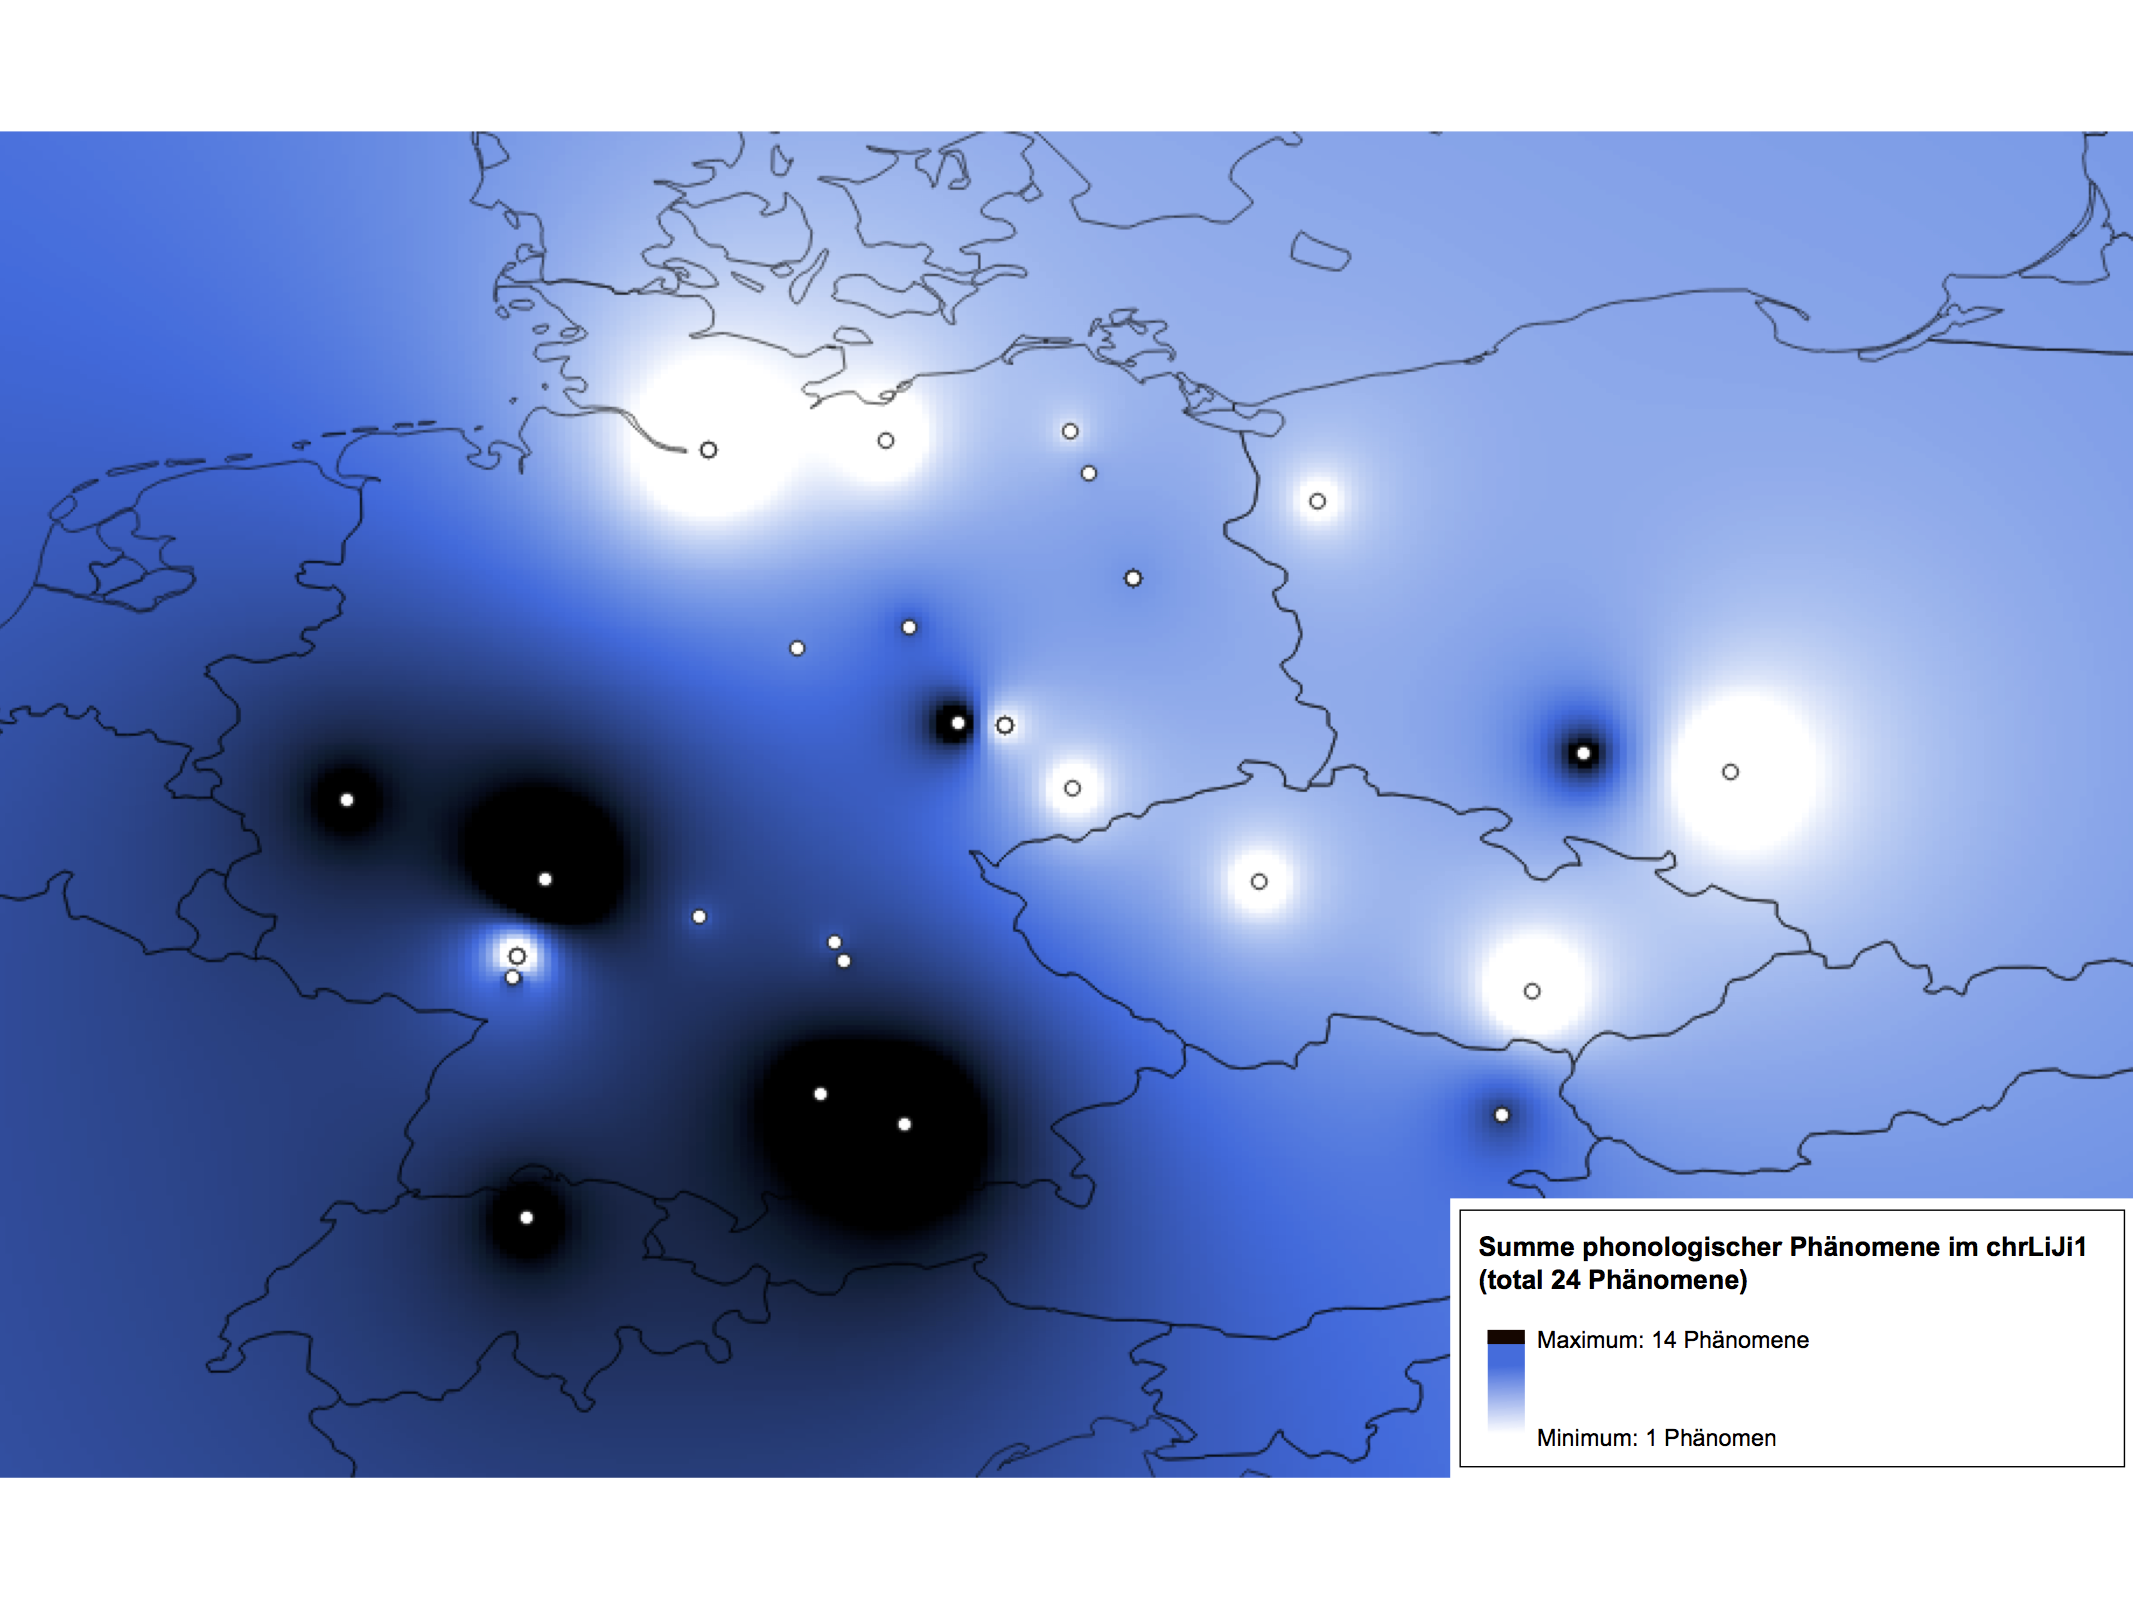
\includegraphics[width=0.32\textwidth]{figures/phon_IDW.png}}
\subfloat[\hai{IDW} \isi{Morphologie}]{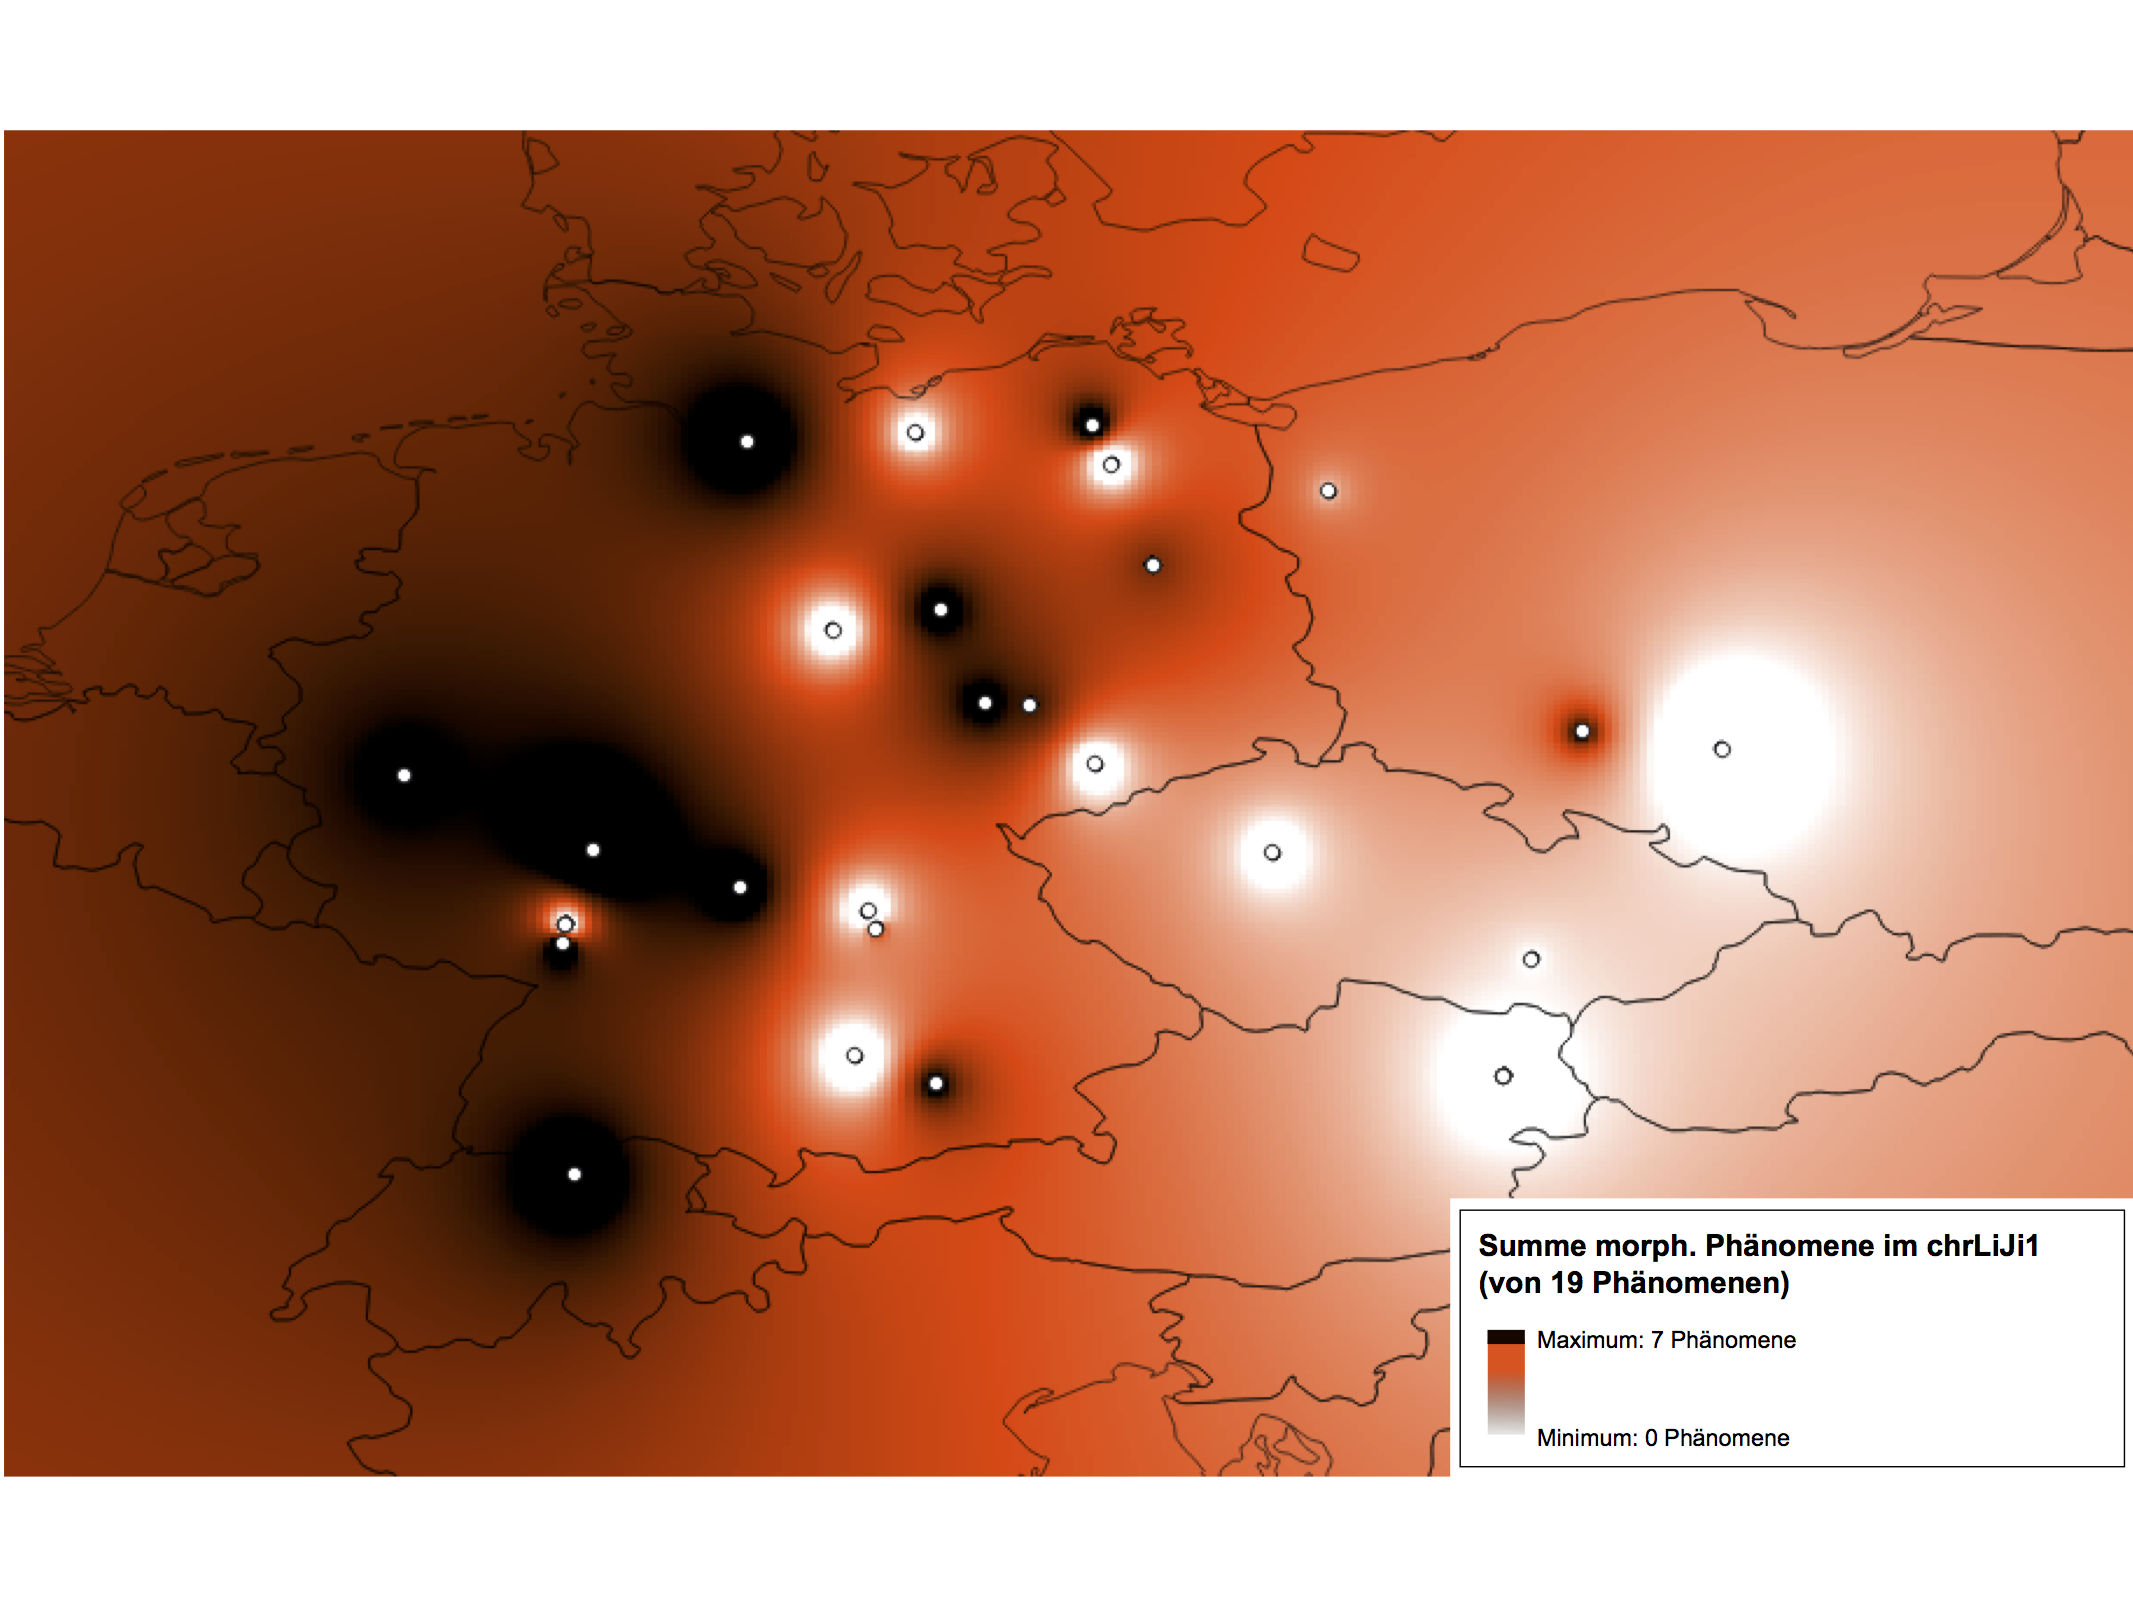
\includegraphics[width=0.32\textwidth]{figures/morph_IDW.png}}
\subfloat[\hai{IDW} \isi{Syntax}]{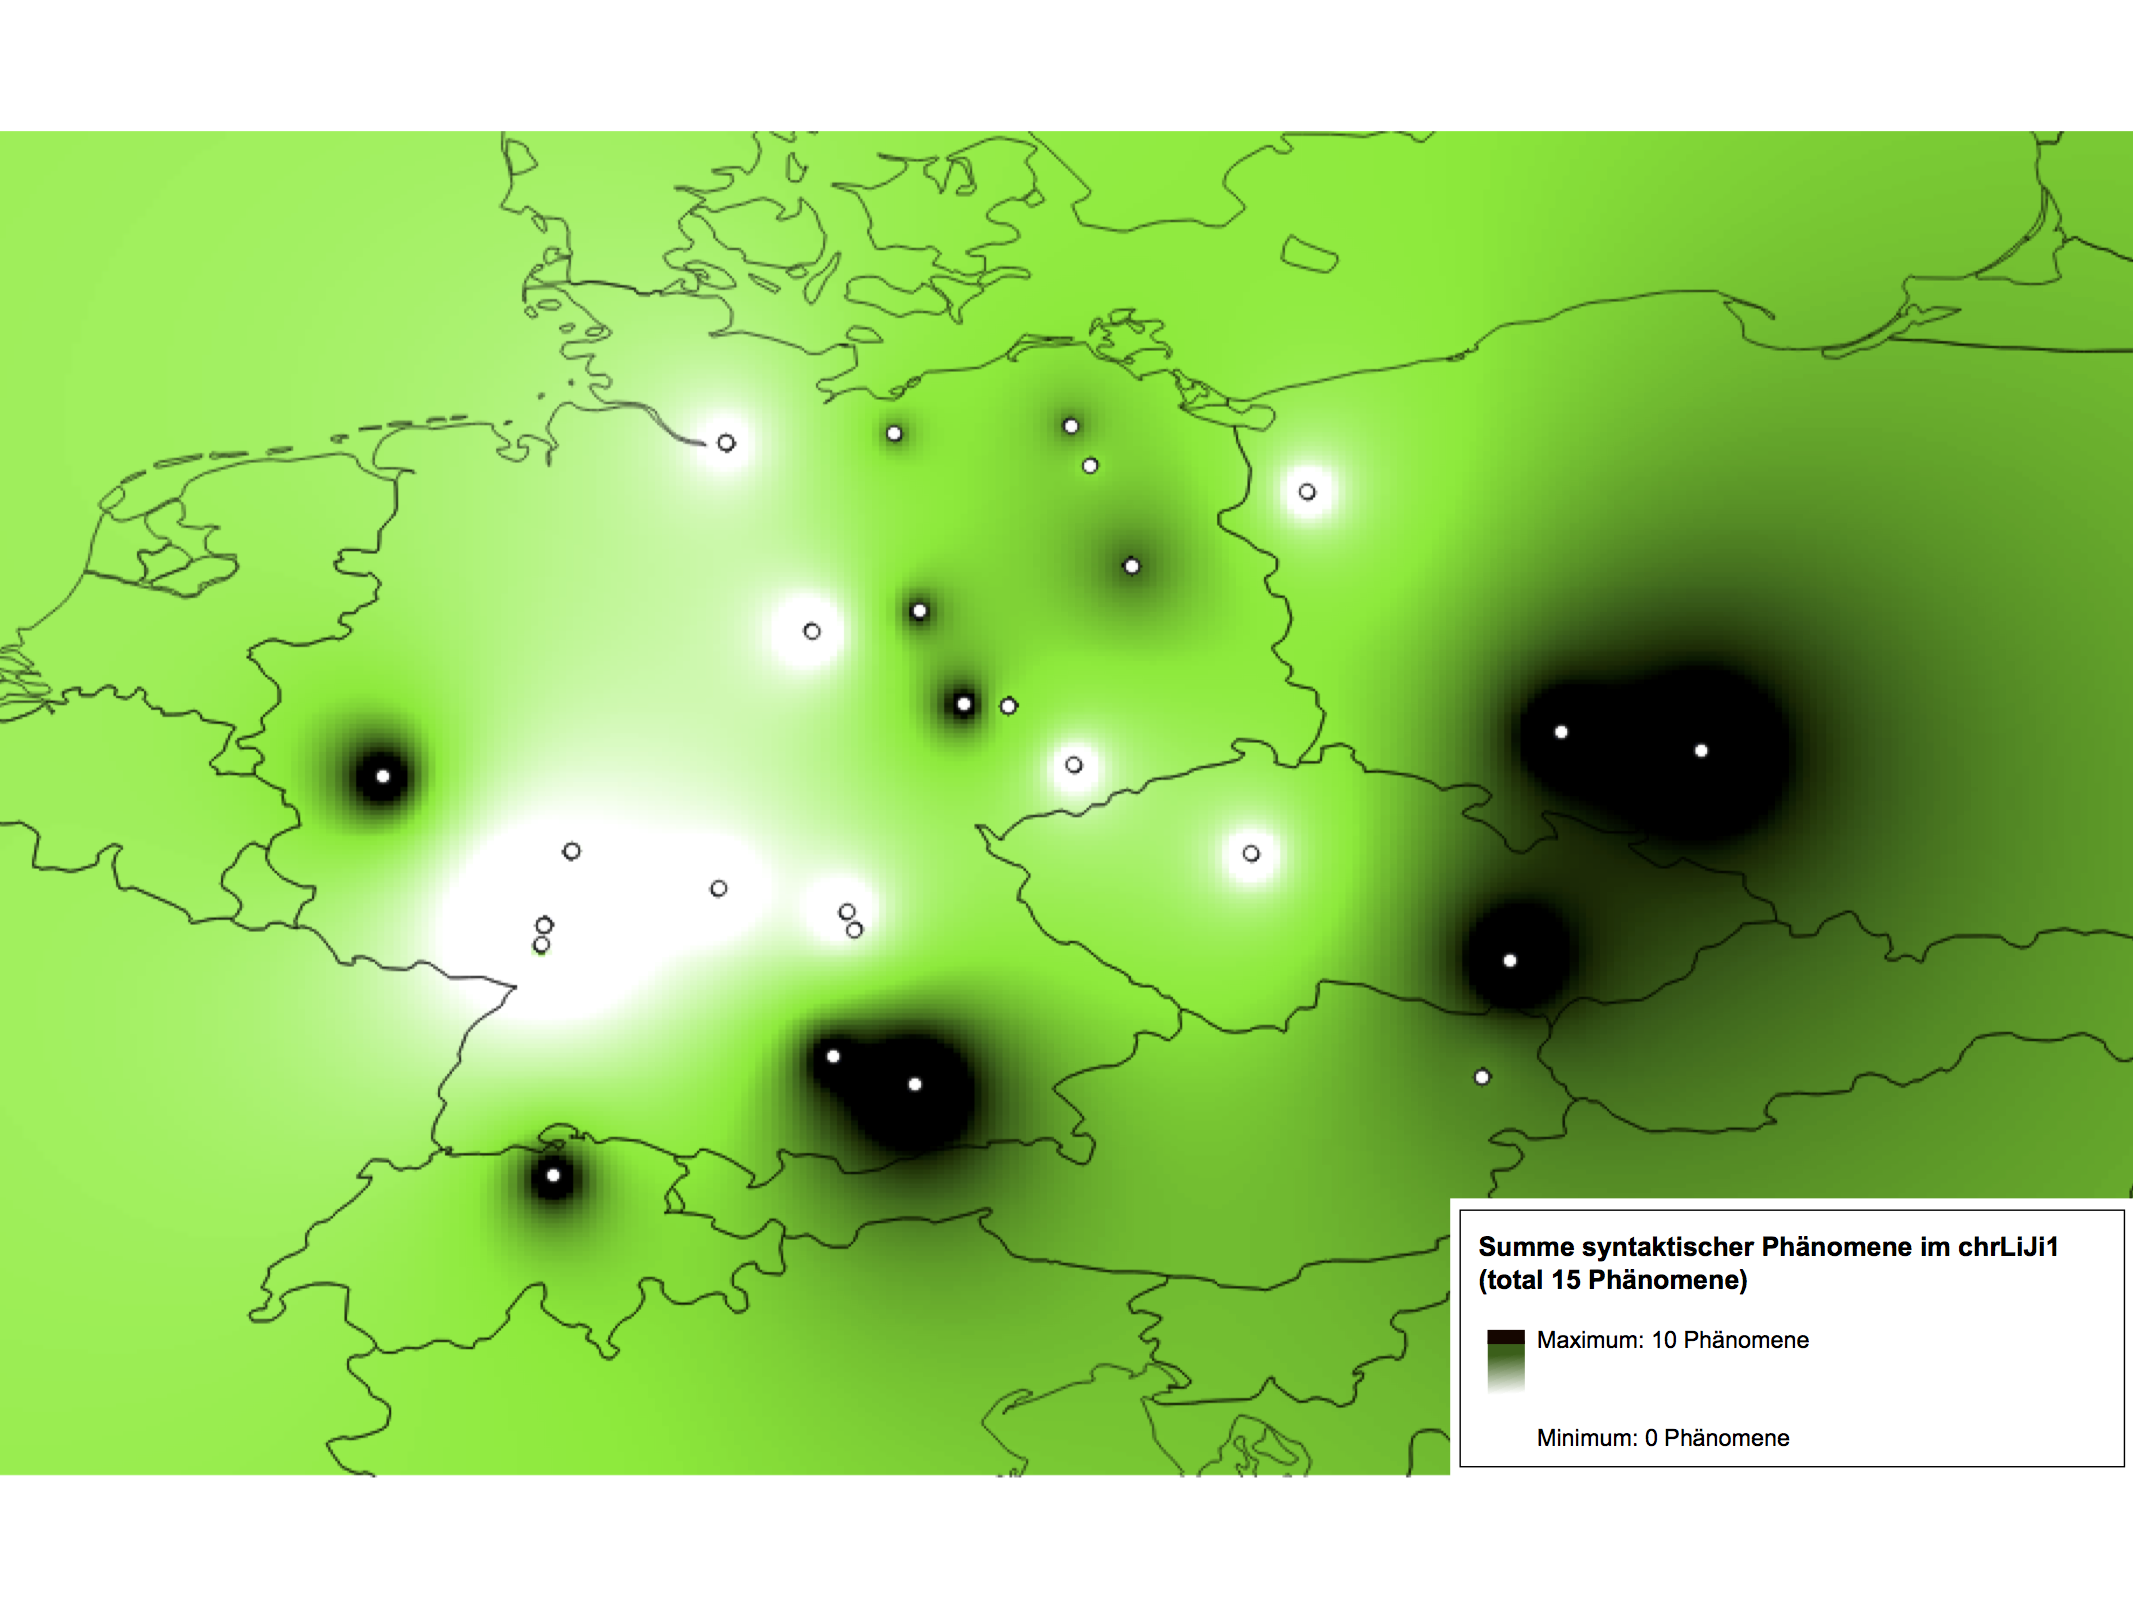
\includegraphics[width=0.32\textwidth]{figures/syn_IDW.png}}
\hfill
\subfloat[\hai{IDW} aller Phänomene]{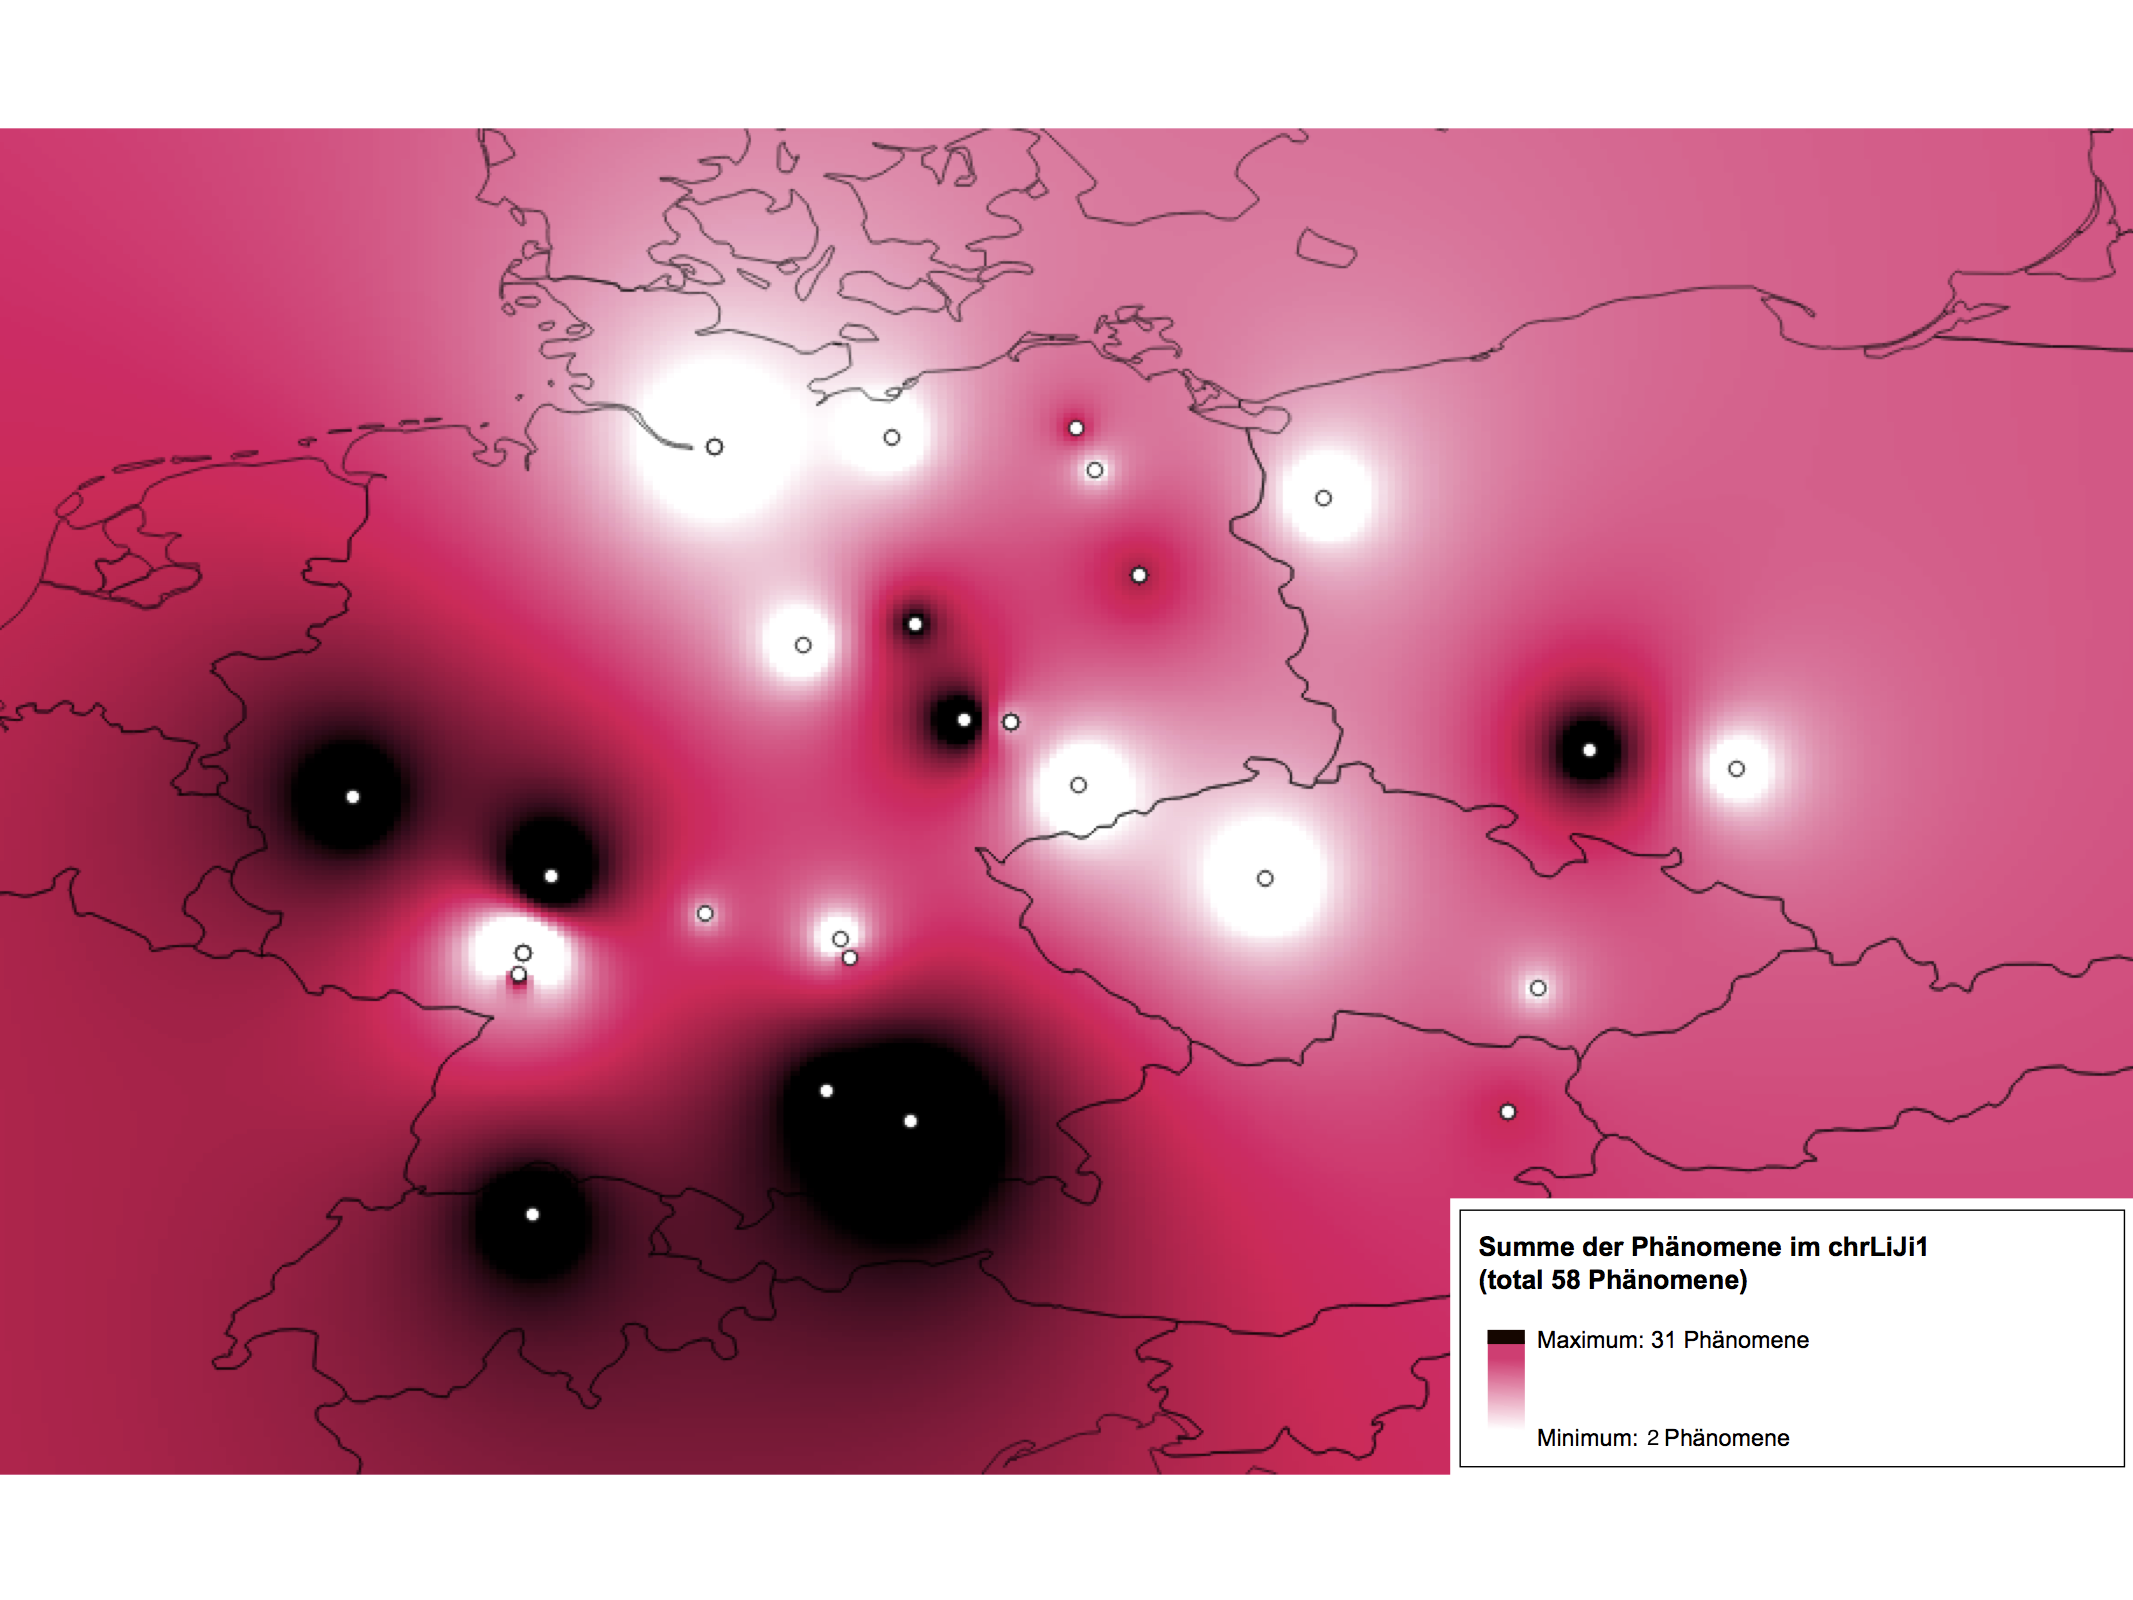
\includegraphics[width=0.99\textwidth]{figures/all_IDW.png}}
\caption{Phänomene im \hai{chrLiJi1} (\hai{IDW} berechnet mit \hai{QGIS})}
\label{alleIDWs}
\end{figure}



 
Das Diagramm in Abbildung \ref{boxplotsummephaen} illustriert die Verteilung der Häufigkeiten der Phänomene innerhalb des \hai{chrLiJi1}-\isi{Korpus}. Die in den meisten Quellen auftretenden Phänomene zur Figurenmanipulation betreffen den \isi{Vokalismus} und die Wortstellung, wohingegen morphologische Eingriffe nur eher singuläre Ereignisse darstellen. Der in 36 Quellen vertretene, aus \hai{V22} ({\mhd} \textit{ê}, \textit{œ}) hervorgegangene Diphthong /ei/ ist die im \isi{Korpus} häufigste Strategie der sprachlichen Markierung jüdischer Figuren. Gefolgt von der \textit{a}-Verdumpfung (in 34 Quellen gegeben), der Monophthongierung von \hai{V24} ({\mhd} \textit{ei}) und der Extrapositionierung voller \hai{{\NP}}s (in jeweils 31 Quellen gegeben). Damit machen Phänomene des \isi{Vokalismus}, der Verbsyntax und Variationen der Grundwortstellung den überwiegenden Anteil an Manipulationsstrategien \,%rs Manipulationsstrategien
 aus. Weniger populär sind Manipulationen des \isi{Konsonantismus} sowie der Nominalsyntax und Nominalmorphologie.


Die Verteilung der Phänomene über die Quellen zeigt in Abbildung \ref{boxplotsummephaen} (S.\, \pageref{boxplotsummephaen}), wie auch das komplementäre Bild in Abbildung \ref{DiagrammSummePhaen} (S.\, \pageref{DiagrammSummePhaen}), dass sich Quellen unterschiedlicher Strategien bedienen und es nicht das \textit{eine} einheitliche \ili{Literaturjiddisch} gibt, sondern nur einige wenige Phänomene regelmäßig in den Quellen vertreten sind. Dennoch  lassen sich wiederkehrende Strukturen erkennen, sobald man die gewonnenen Daten clustert. Die Ward-Clusterung der im \hai{chrLiJi1} auftretenden Phänomene untereinander (Abbildung \ref{boxplotclusterphaen}) ergab vier Hauptcluster, die zeigen, welche Phänomene gemeinsam auftreten. Erstaunlich verhalten sich die Phänomene der Cluster \hai{C} und \hai{D}: Während Cluster \hai{D} ausschließlich vokalische Phänomene beinhaltet, die für das Westjiddische charakteristisch sind, besteht Cluster \hai{C} vorwiegend aus Extrapositionen und Phänomenen, die im Verdacht stehen, \hai{{\VO}}-Strukturen emulativ abzubilden. Diese zwei Cluster sind damit auf sprachliche Strukturen zurückzuführen, die auch in natürlichen Sprache (insbes. im gesprochenen Westjiddischen) gemeinsam auftreten. In den beiden übrigen Clustern \hai{A} und \hai{B} ist keine solche Homogenität der Phänomene zu erkennen. Die Clusterung der Phänomene zeigt vor allem in den Unterclustern, dass Phänomene des gleichen Typs auch gemeinsam auftreten;\, so z.\,B.\, im Fall der Rundungen und Entrundungen (/y/ > /i/, /∅/ > /e/, /o/ > /u/, /u/ > /o/, \hai{V34}) in einem Untercluster von Cluster \hai{B}.

 \begin{figure}
\centering
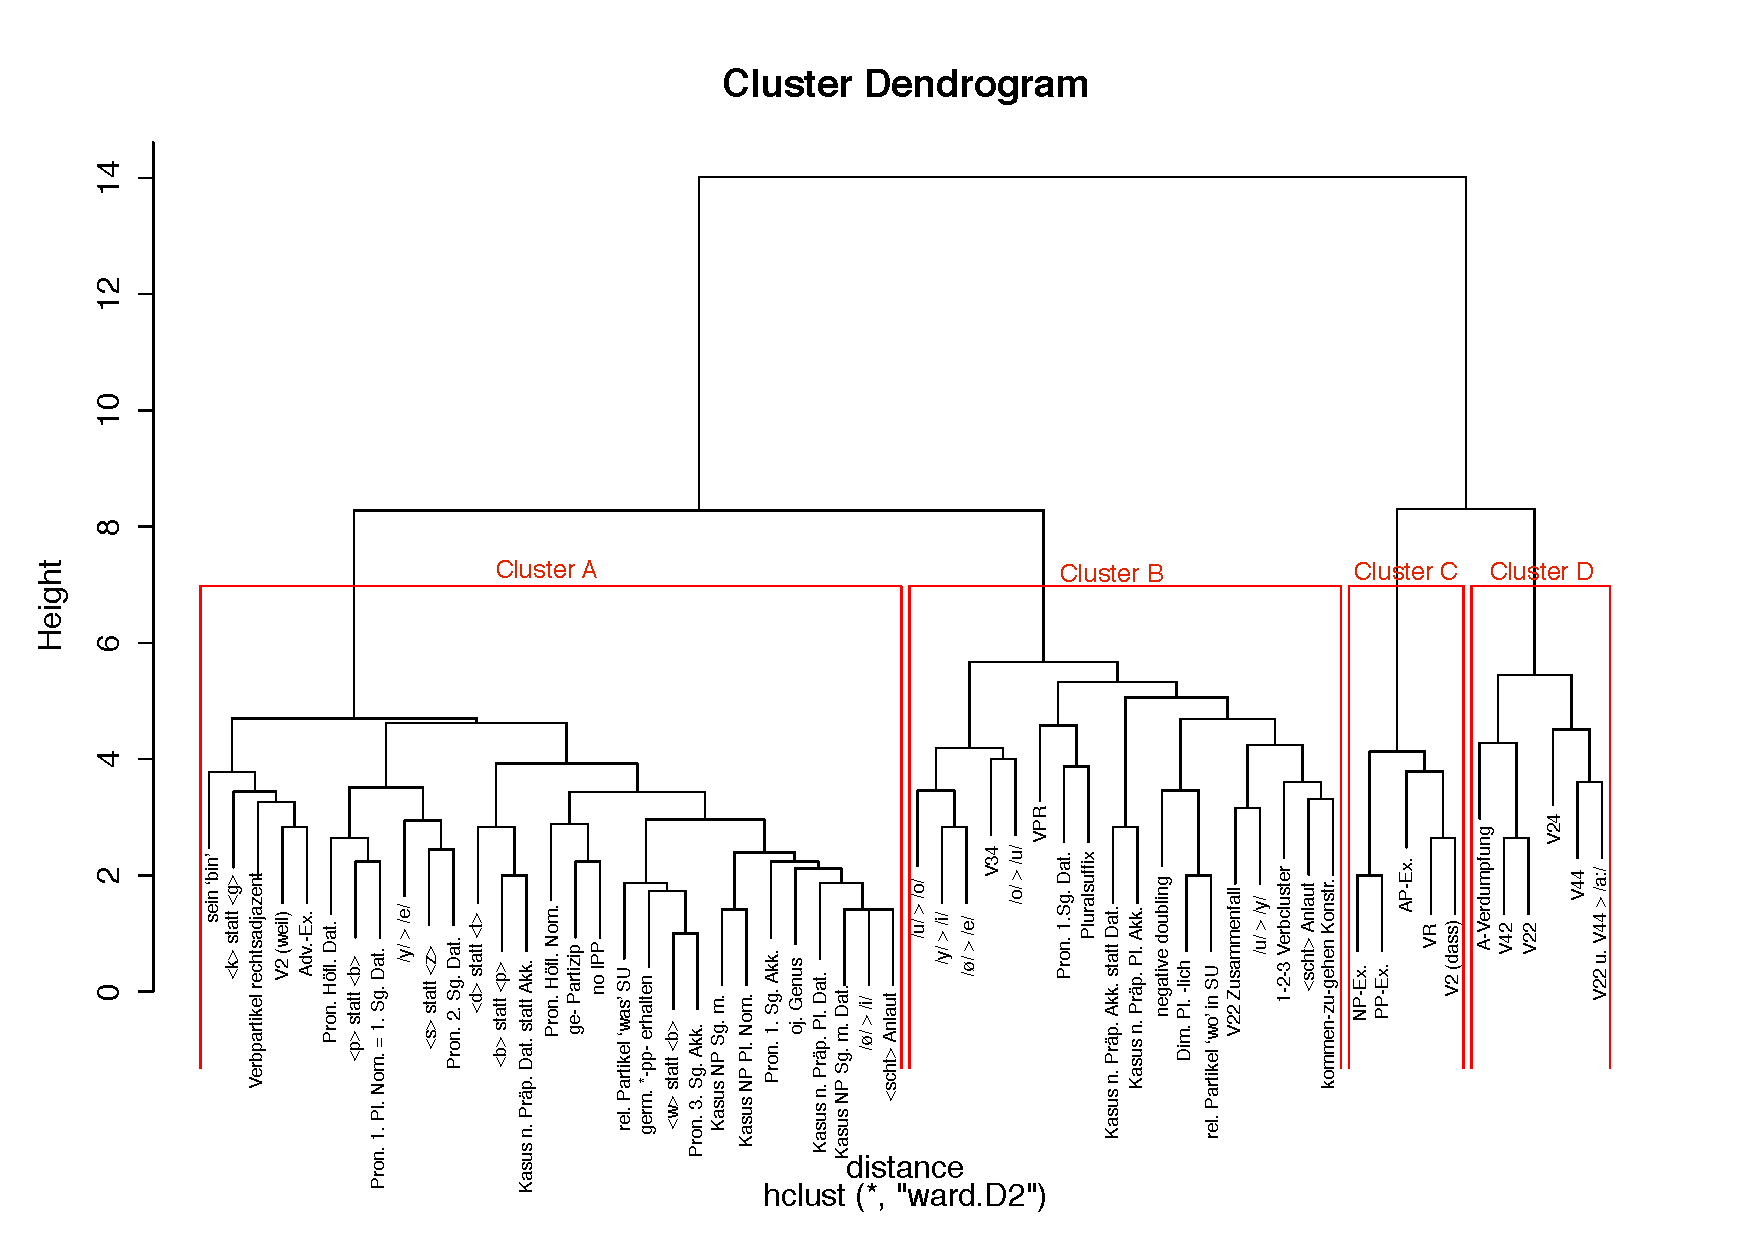
\includegraphics[width=\textwidth]{figures/Rplot_phaen.pdf}
		\caption{\label{boxplotclusterphaen} Ward-Cluster aller im \hai{chrLiJi1} auftretenden Phänomene}
	\end{figure}
 
 

\begin{figure}
\centering
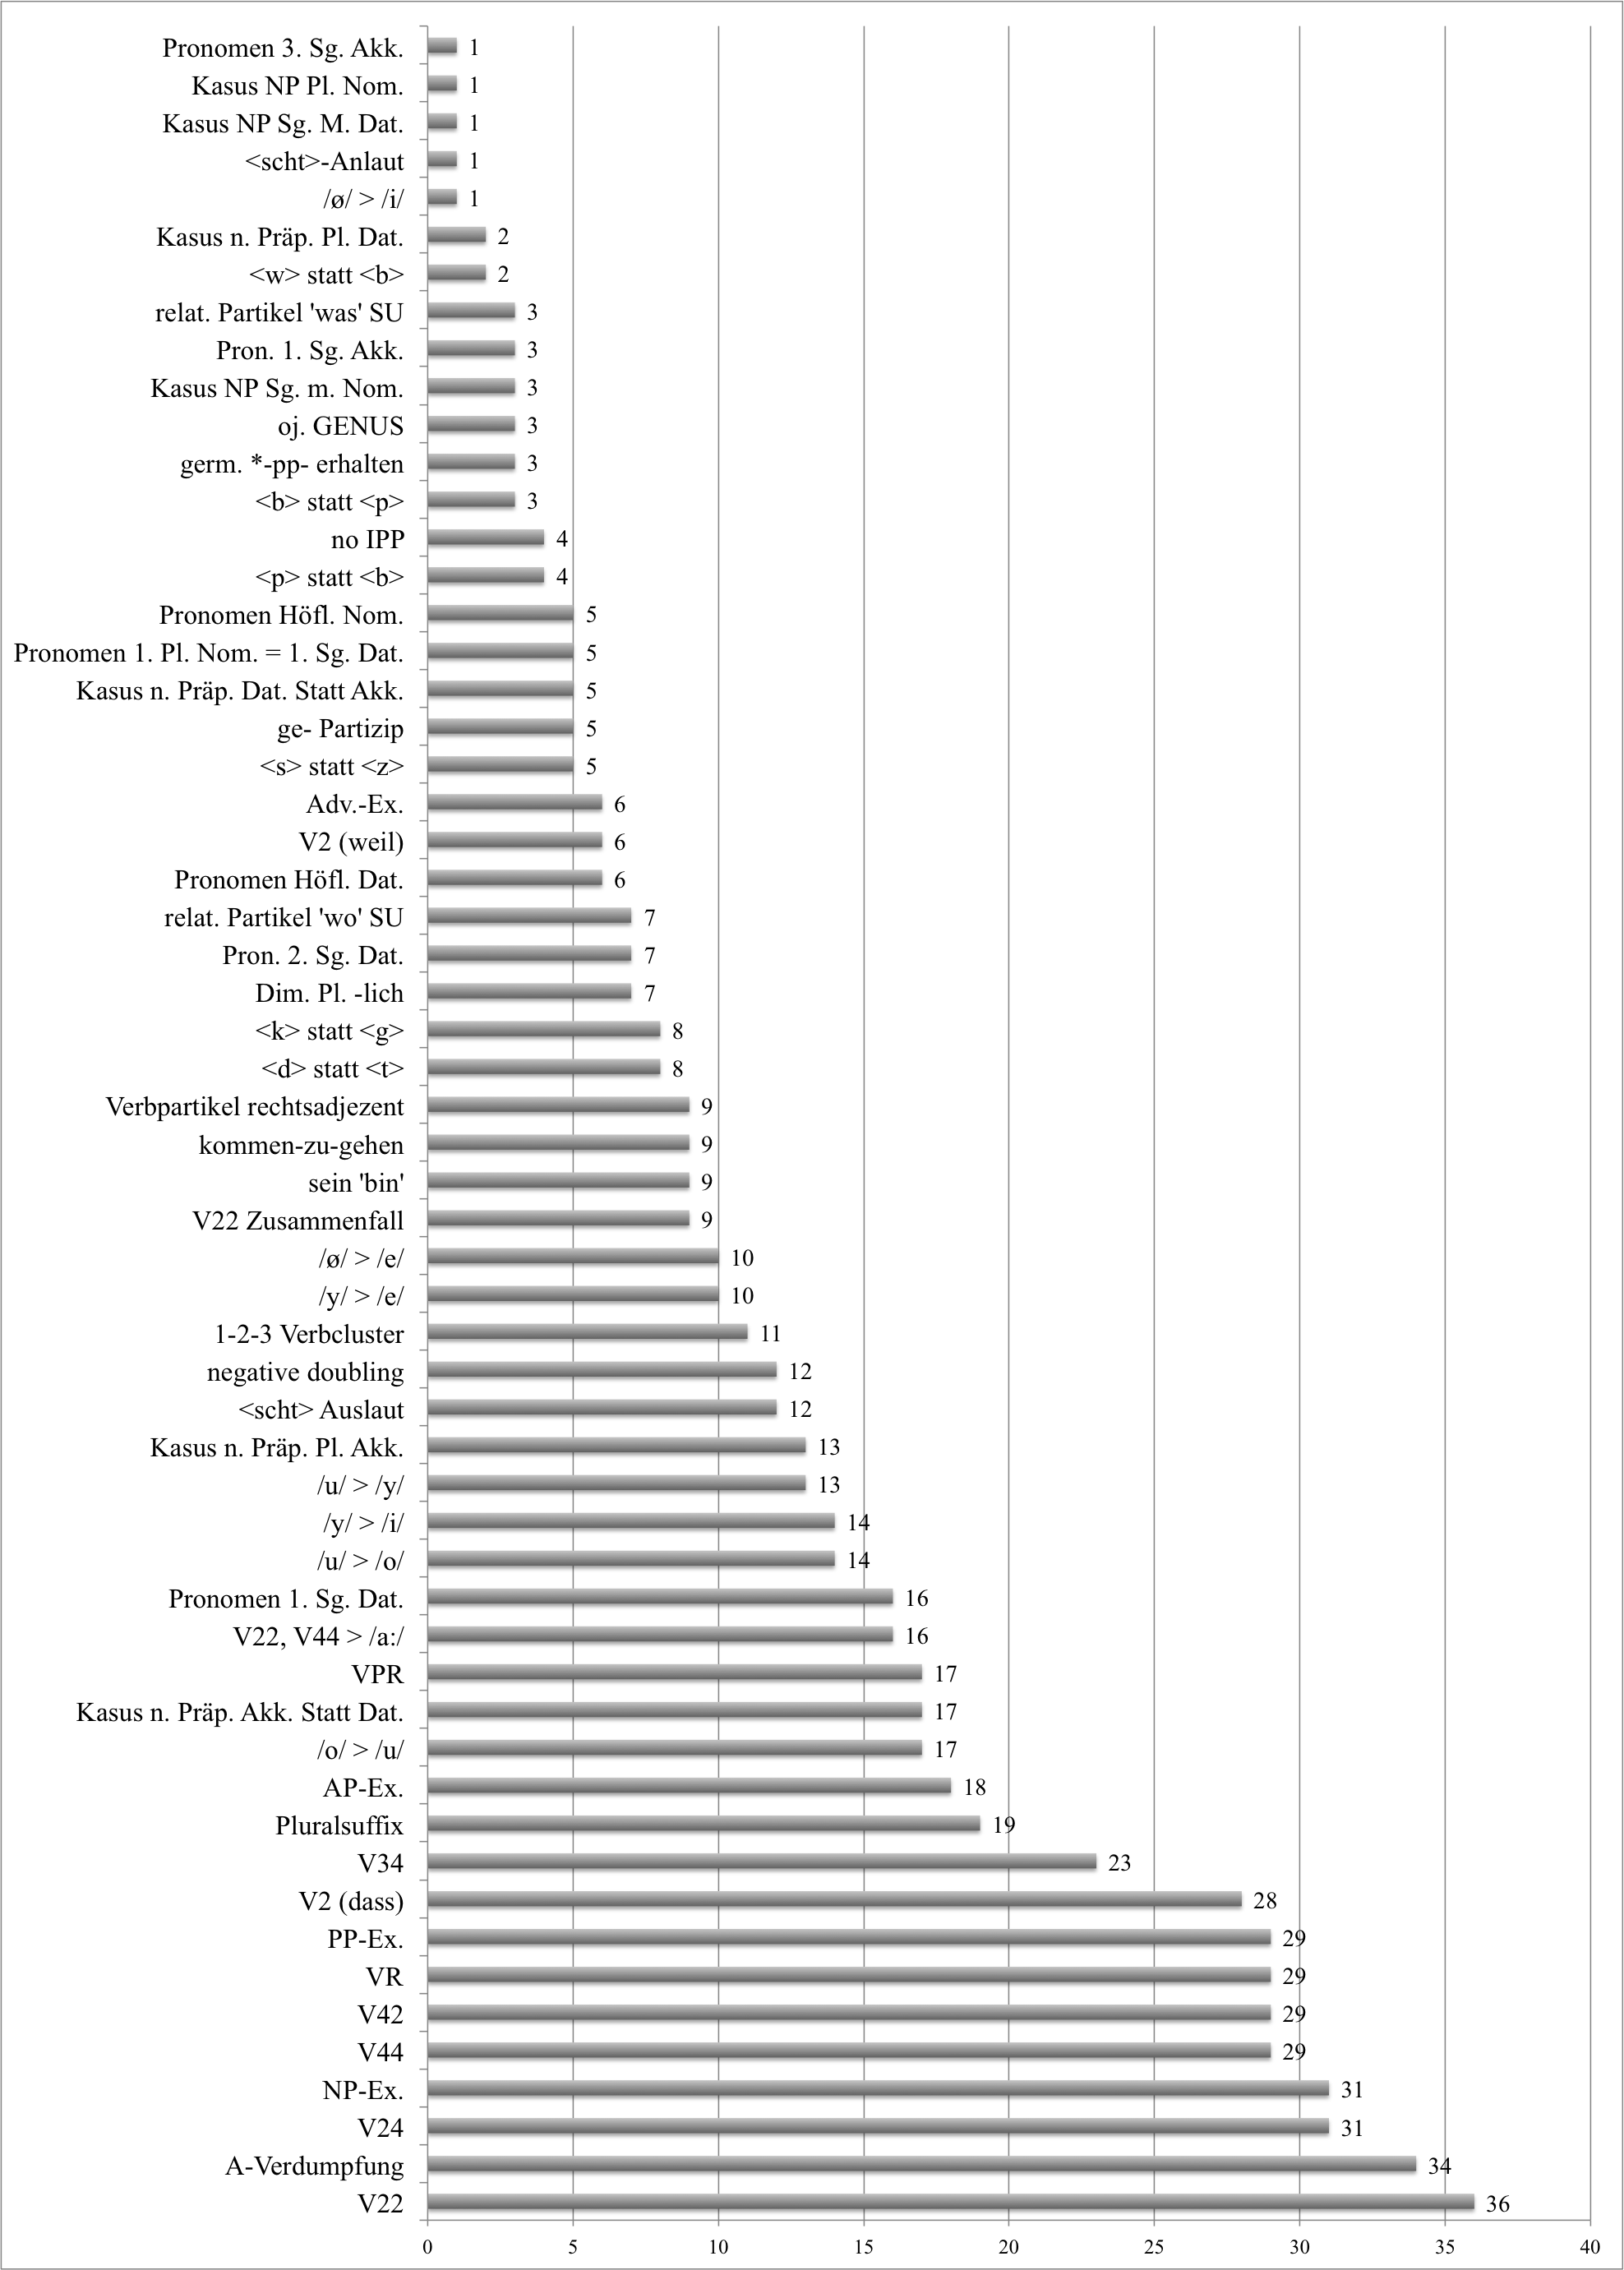
\includegraphics[width=\textwidth]{figures/SUMMEPHAE4.png}
		\caption{\label{boxplotsummephaen} Häufigkeit aller im \hai{chrLiJi1} auftretenden Phänomene}
	\end{figure}
 
 
 
 \section{Distribution der Phänomene innerhalb der einzelnen Quellen}\label{clusterQuellen}
%\noindent
Die folgenden Daten entsprechen denen aus Kapitel \ref{clusterPhänomene}\, mit dem Unterschied, dass nun die beiden Achsen (Phänomene/Quellen)\, transponiert wurden (vgl. die Tabelle im Anhang S.\, \pageref{appendixphaenall}). So lassen sich nun Aussagen darüber treffen, wie sich die einzelnen Quellen bezüglich der verwendeten Phänomene verhalten.

\newpage 
Der Durchschnitt liegt bei 13 unterschiedlichen Manipulationsstrategien pro Quelle, bei einer Standardabweichung von 7.  Die Spannbreite zwischen Quellen, die viele bzw. wenige Phänomene zur sprachlichen Charakterisierung nutzen, ist groß. Wie das Diagramm in Abbildung \ref{DiagrammSummePhaen} zeigt, unterscheiden sich die Quellen des \hai{chrLiJi1}-\isi{Korpus}, was die Vielfalt der Phänomene betrifft, stark. 
 
 \begin{figure}
\centering
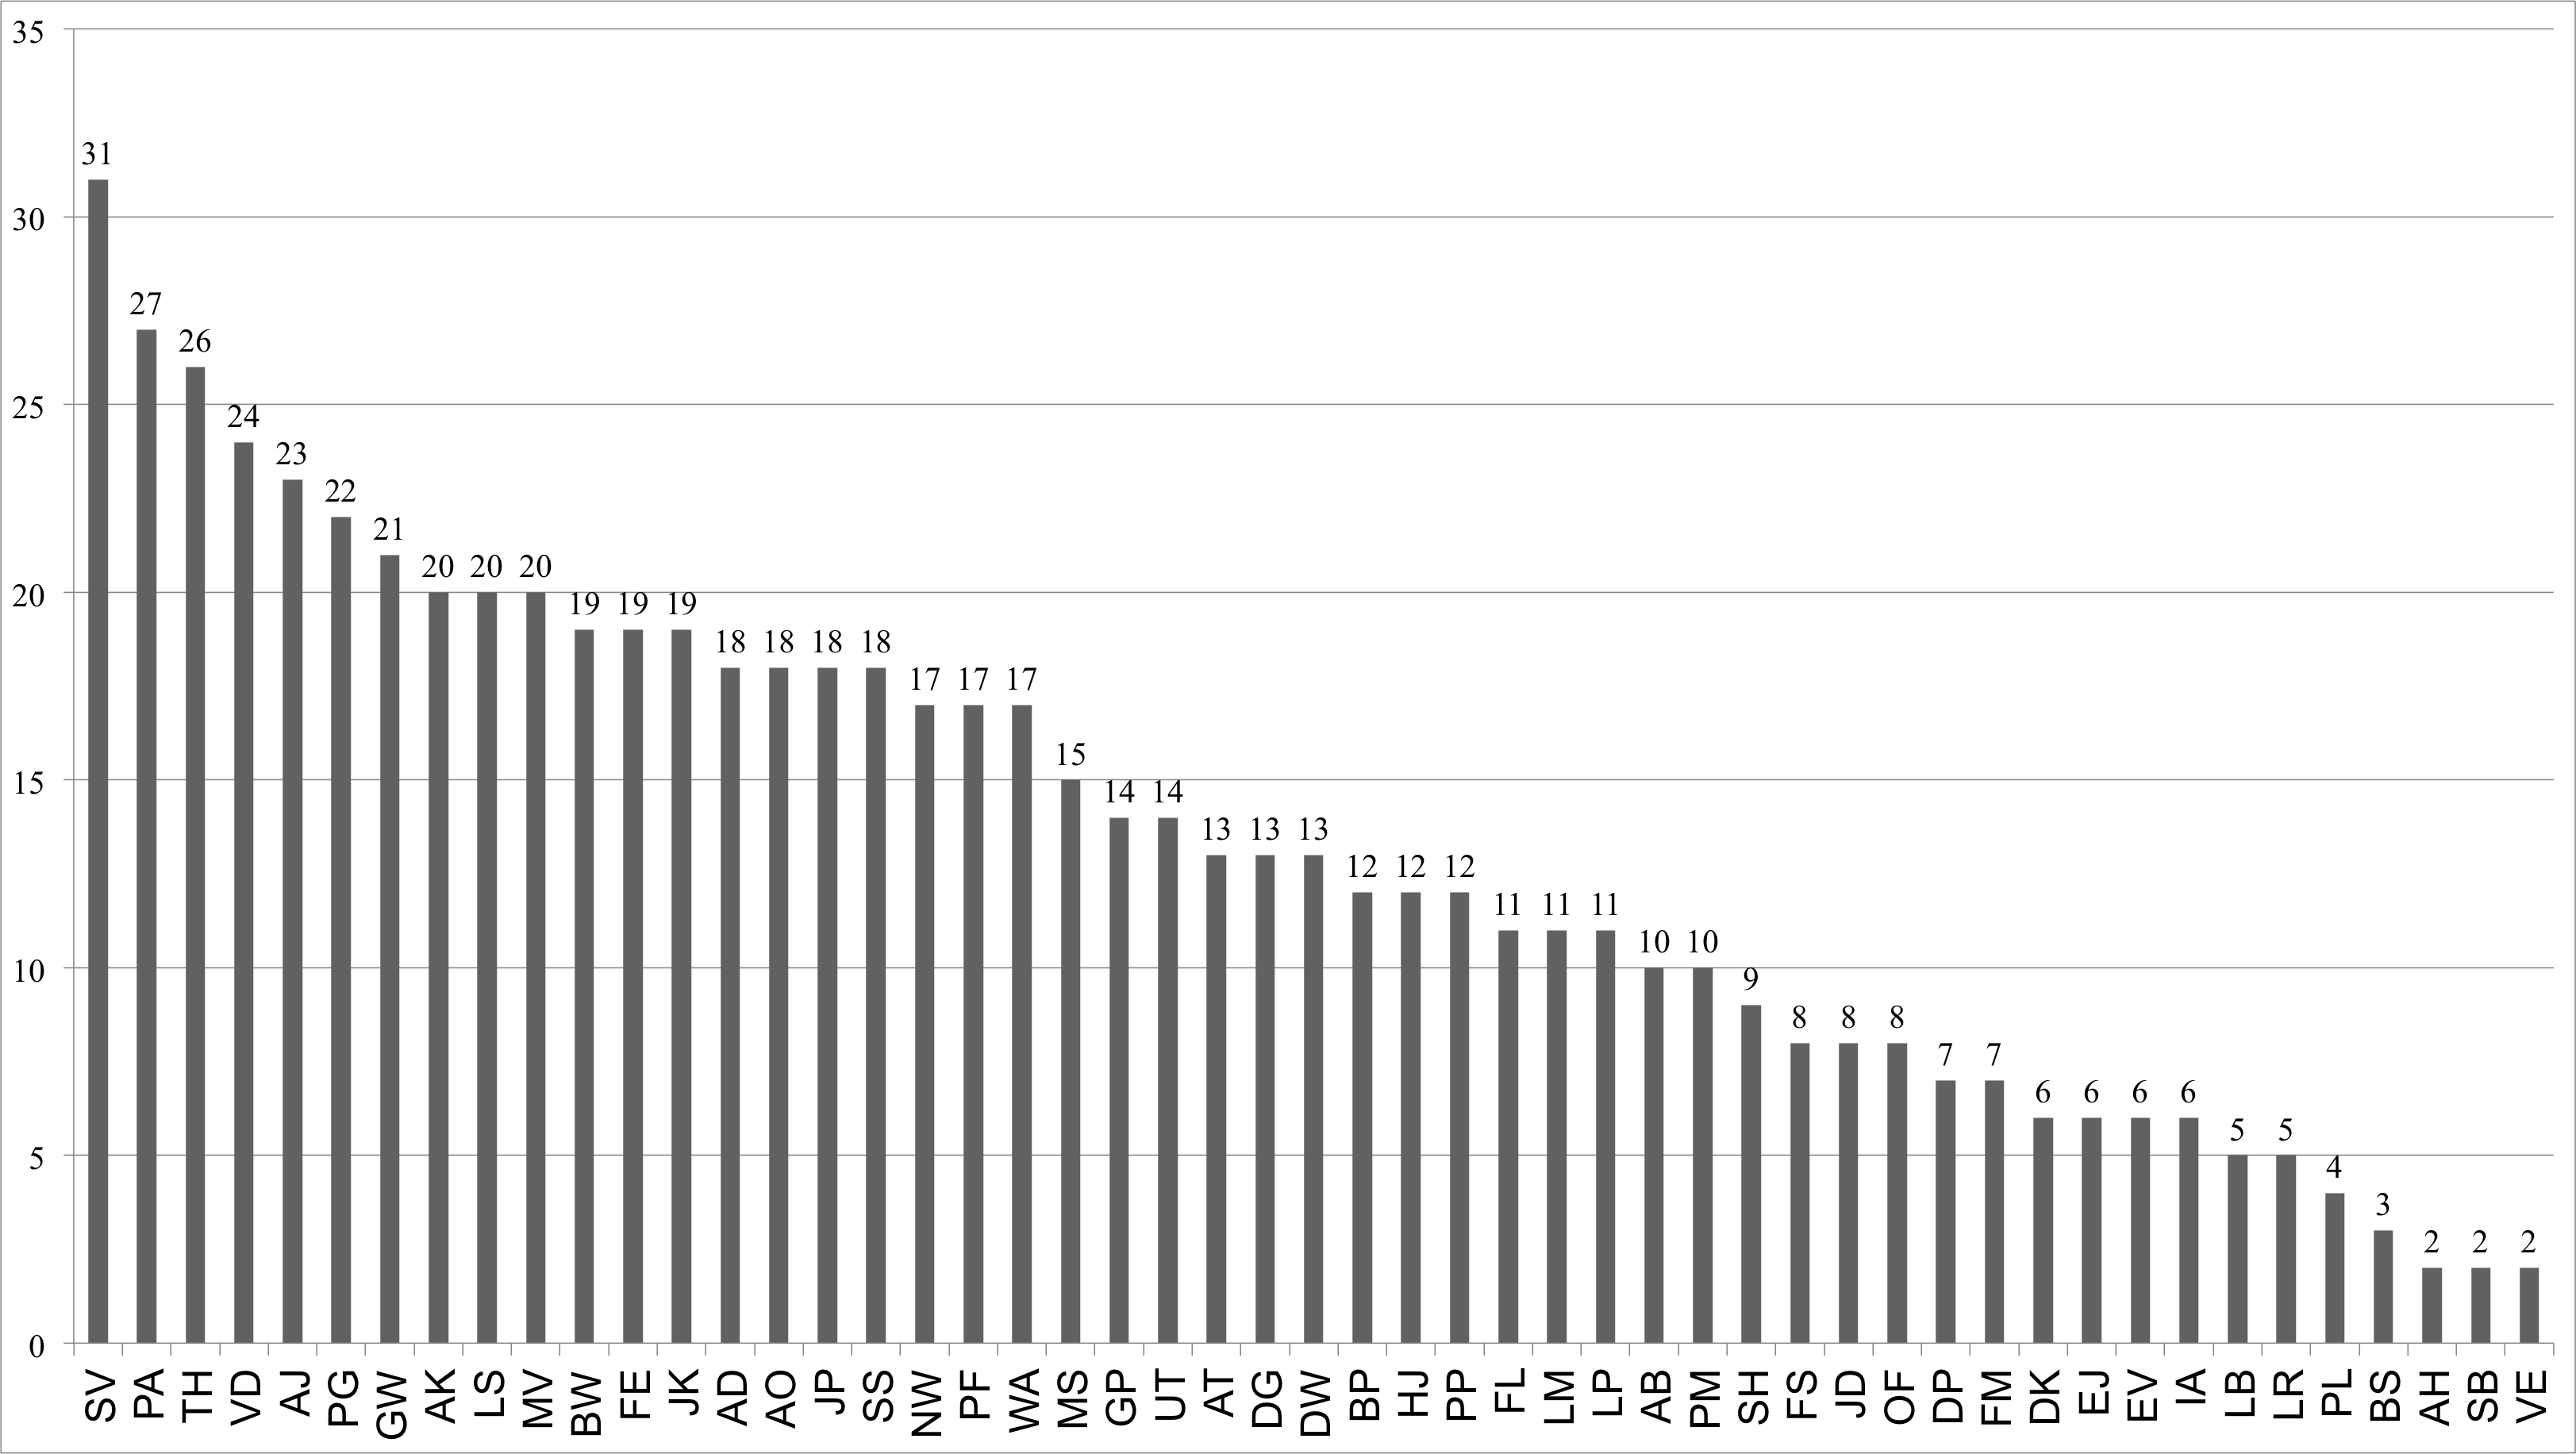
\includegraphics[width=\textwidth]{figures/DiagrammSummePhaen.png}
		\caption{\label{DiagrammSummePhaen} Quellen des \hai{chrLiJi1} nach Summe der Phänomene}
	\end{figure}
 

 

Das areale Bild der Phänomenhäufigkeit zeigt, dass sich Quellen mit der höchsten Phänomenvielfalt in Berlin, Leipzig, Frankfurt und München, und damit besonders in Großstädten, finden. Die Kartierung der Quellen nach ihrer Phänomenhäufigkeit in Abbildung \ref{summepaenomenequellen} zeigt, dass vor allem Quellen aus dem ländlichen Raum weniger Strategien aufweisen als städtische. %  Besonders Quellen östlich der veranschlagten Hamburg-Bregenz-Achse zeigen mit fünf bis neun Phänomenen eher geringeren Aufwand als Quellen  westlich davon. 

\begin{figure}
\centering
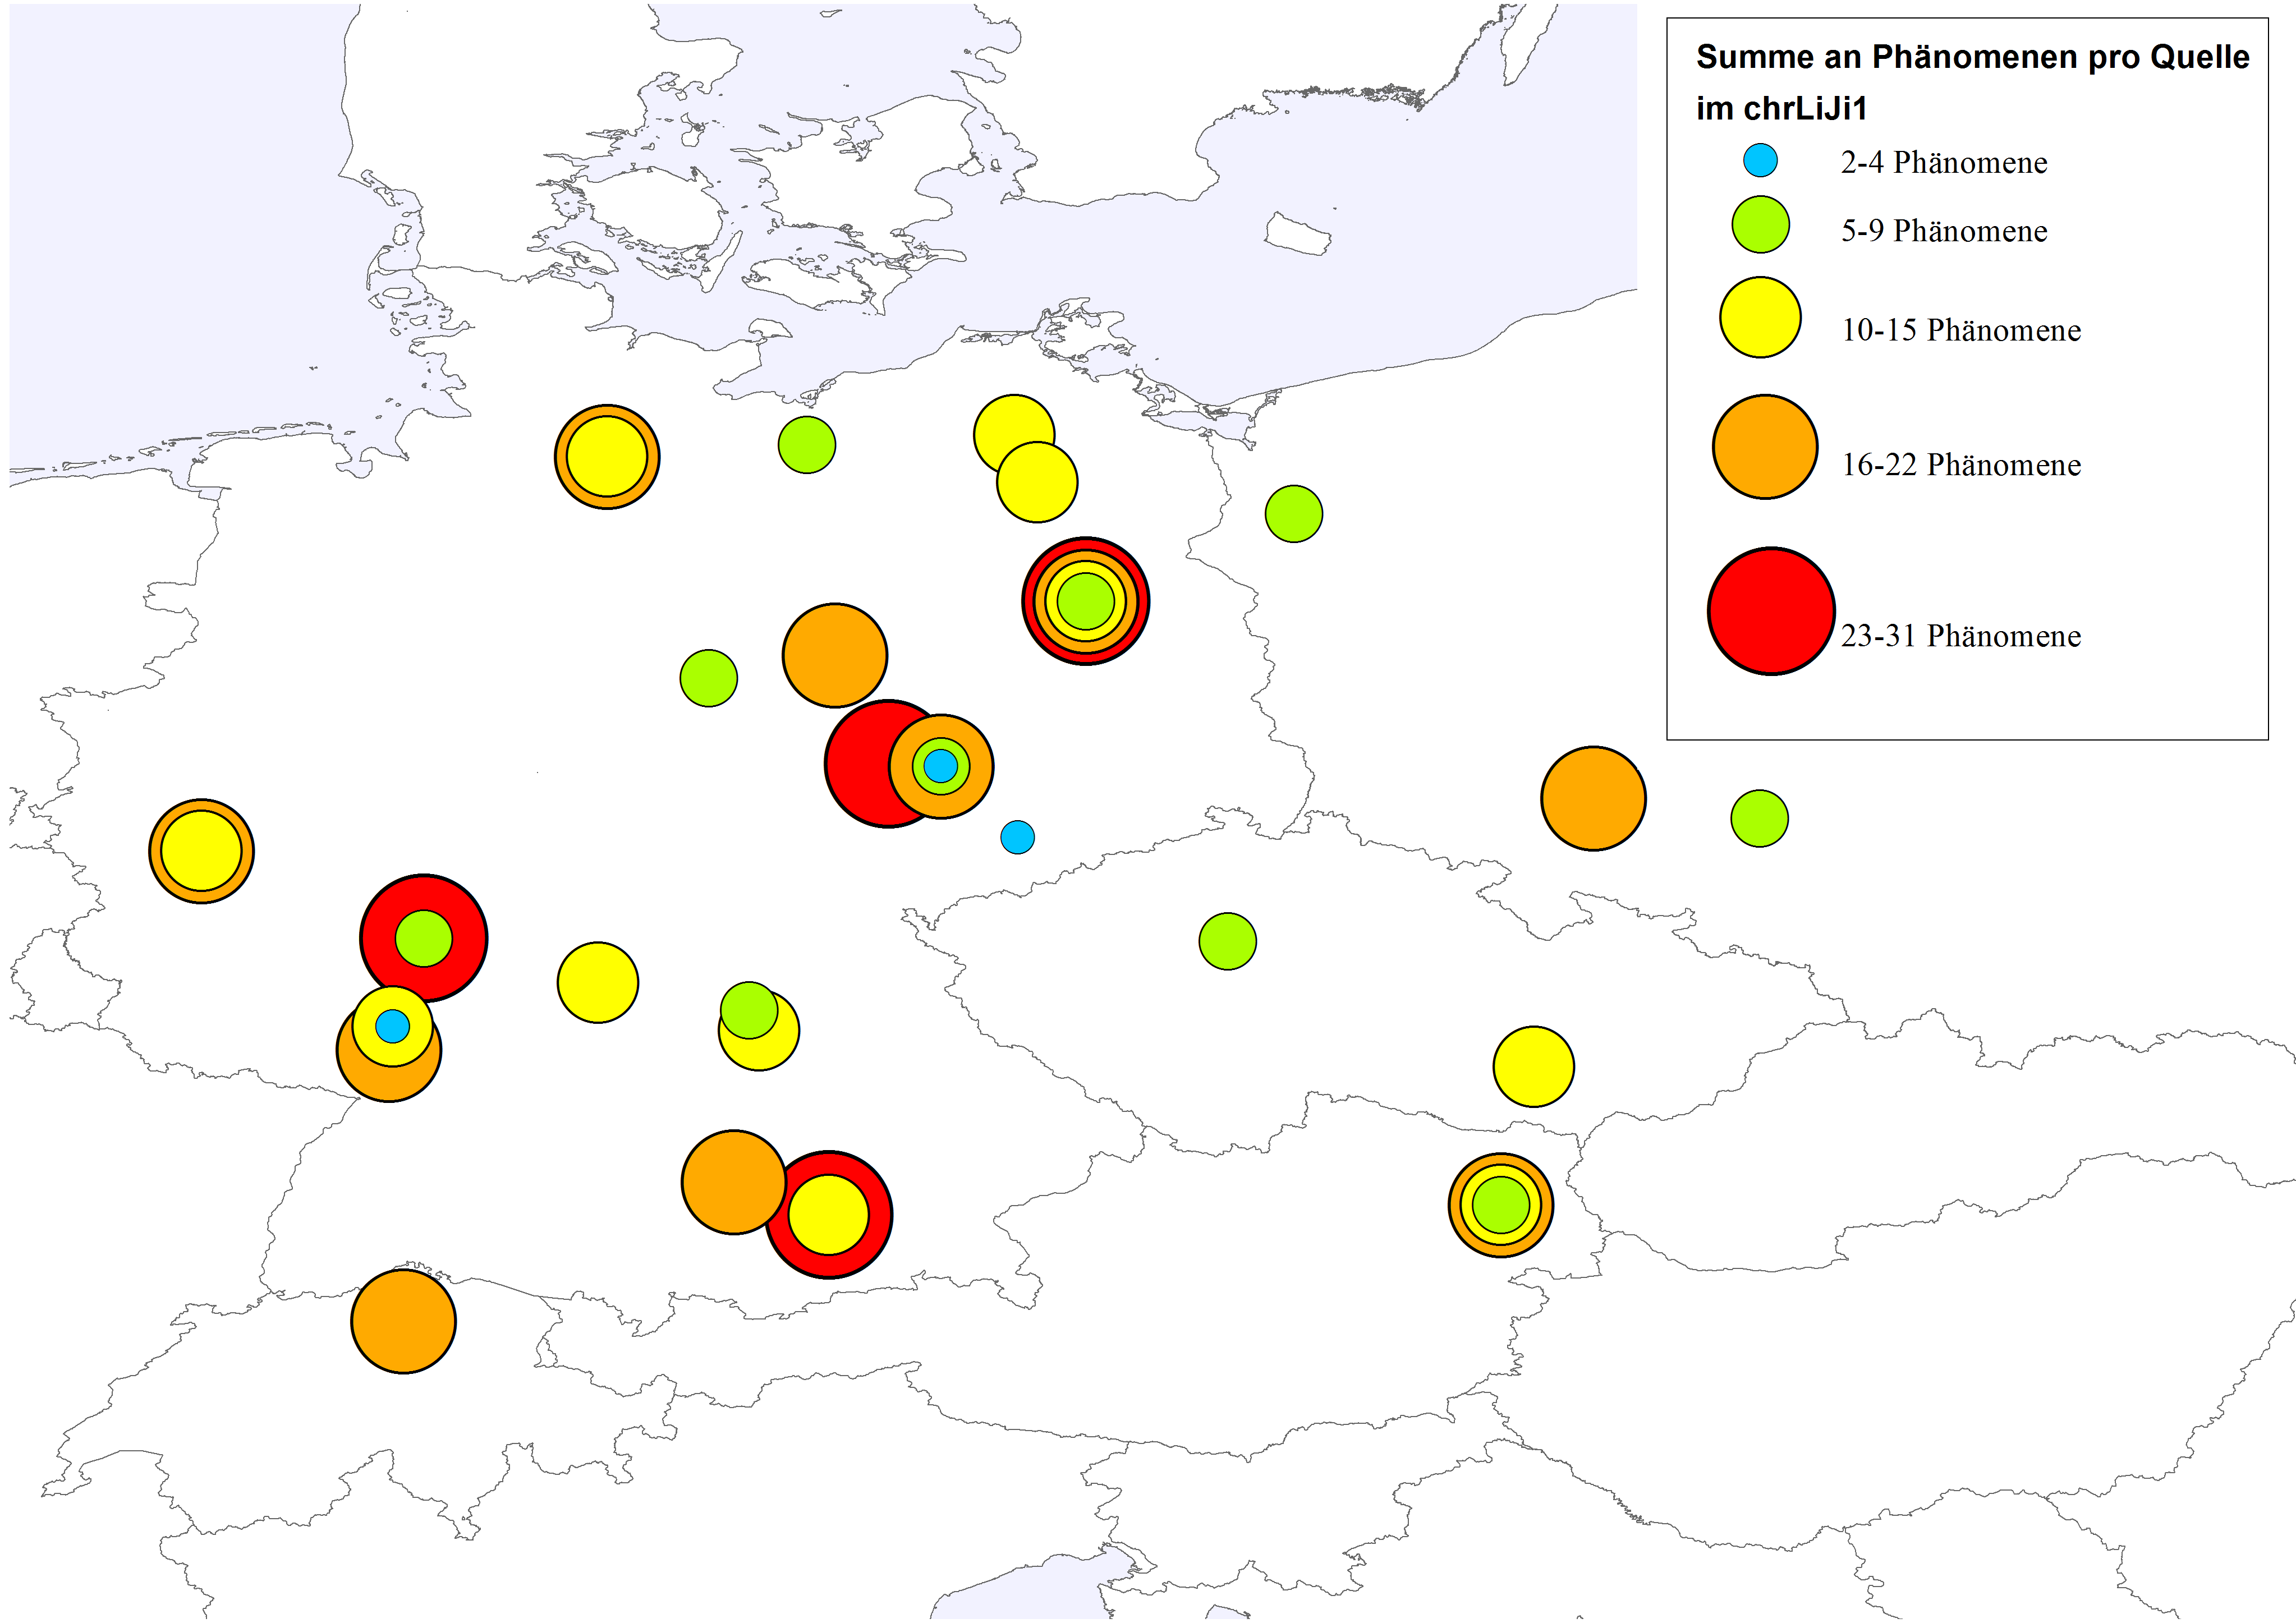
\includegraphics[width=\textwidth]{figures/summepaenomenequellen.png}
		\caption{\label{summepaenomenequellen} Areale Verteilung der Phänomenvielfalt der Quellen des \hai{chrLiJi1}}
	\end{figure}
 


Die Clusteranalyse der Verteilung der Phänomene auf die einzelnen Quellen zeigt, dass es unterschiedliche Strategien zur Figurenmanipulation gibt, derer sich die Quellen bedienen. Würden alle Quellen die gleichen Phänomene aufweisen, so wäre ein solches Bild, wie es Abbildung \ref{boxplotcluster} darstellt, deutlich einheitlicher und weniger verästelt.
  
 
 \begin{figure}
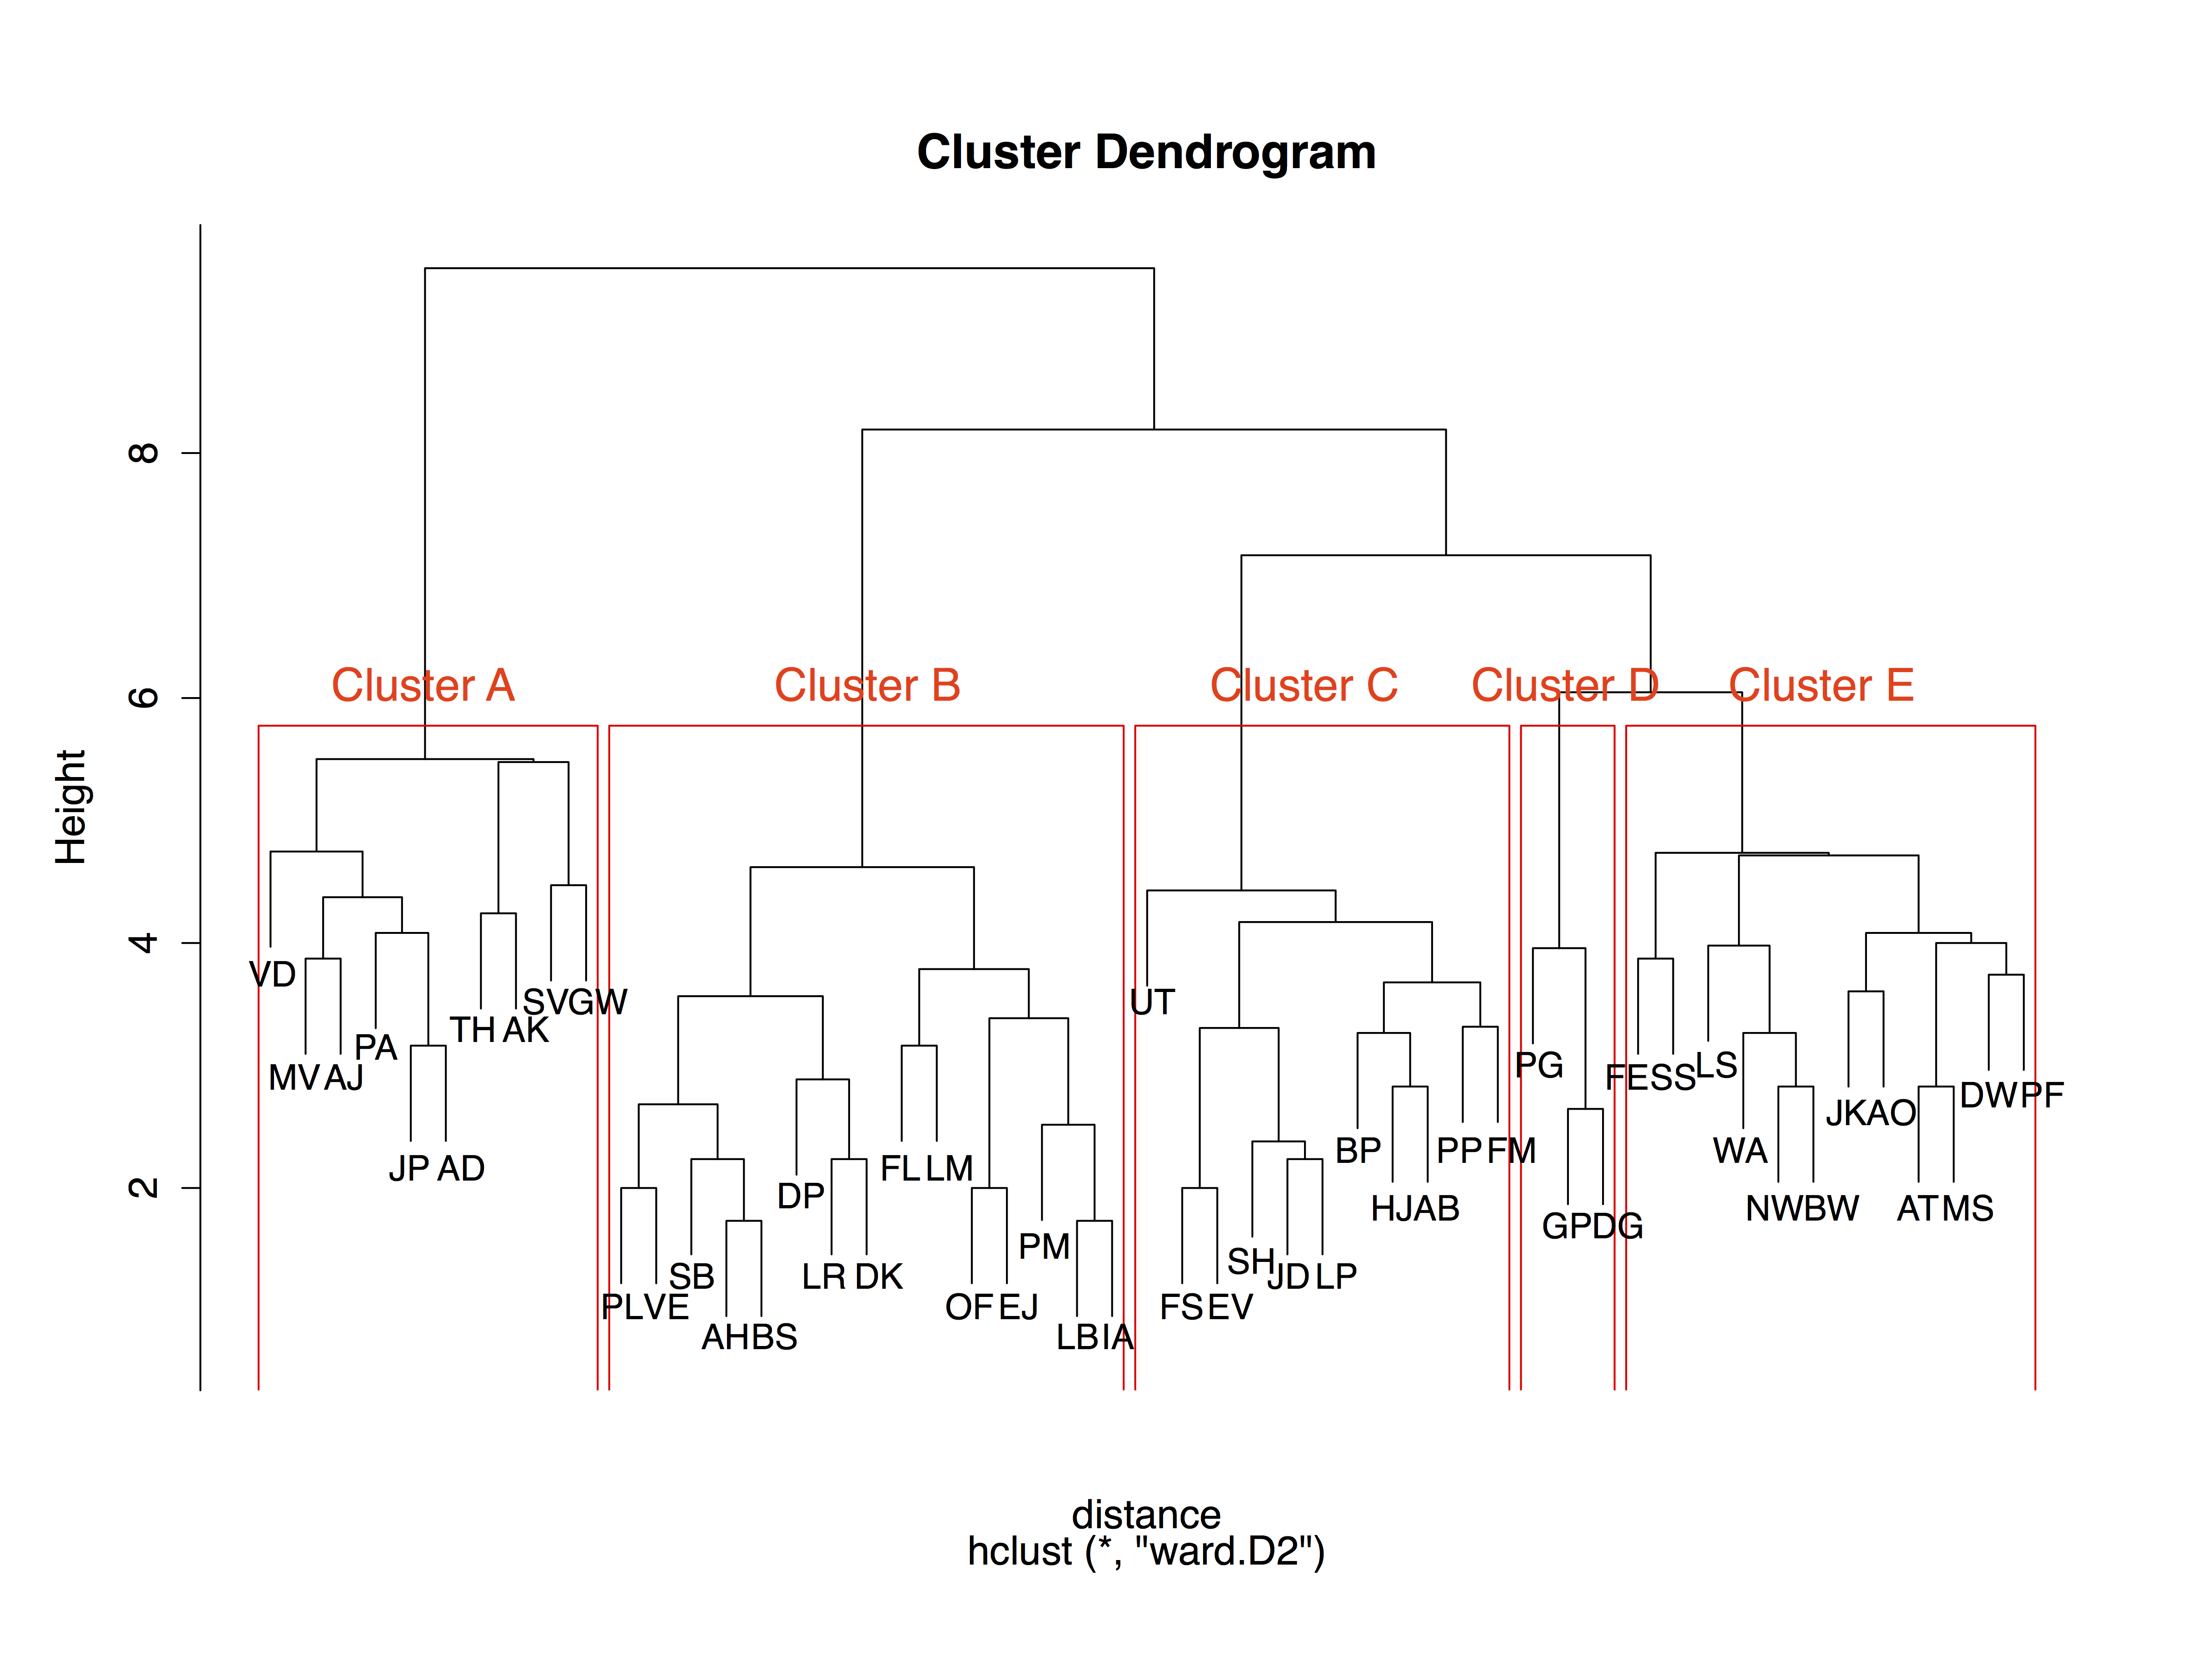
\includegraphics[width=\textwidth]{figures/Rplot_Sources.png}
		\caption{\label{boxplotcluster} Ward-Cluster aller \hai{chrLiJi1}-Quellen nach Phänomenen}
	\end{figure}
 
	
 \largerpage
Die diachrone Verteilung der fünf Hauptcluster (in Abbildung  \ref{boxplotcluster} rot eingefasst) zeigt, dass der Clusterung der Quellen eine soziolinguistisch begründete Systematik zugrunde liegt. Im Histogramm \ref{histoCLUSTERQ} sehen wir, dass die  jeweiligen Cluster \hai{A}, \hai{B} und \hai{C} zumeist in Phasen auftreten. Das heißt, dass die Anordnung im zeitlichen Raum nicht zufällig ist. Bei den Clustern \hai{D} und \hai{E} sind zwar auch gewisse Phasen zu erkennen, in denen sie mehrfach auftreten, im Vergleich zu den drei anderen Clustern streuen diese beiden aber deutlich mehr. Die zeitliche Anhäufung von Quellen desselben Clusters spricht dafür, dass der literaturinterne Diskurs des Literaturjiddischen einen deutlichen Einfluss auf die Wahl der Manipulationsstartegien ausübt. Die meisten Texte nehmen also andere Texte zum Vorbild und dienen zugleich als Vorlage für andere Texte.


\begin{figure}
	\begin{tikzpicture}
		\begin{axis}[only marks, width=0.82\textwidth,height=0.2\textheight,
		legend style={at={(1,1)},xshift=+0.2cm, yshift=-0.0cm,anchor=north west,nodes=left},
 			%title={Funktionstypen des sp\"aten Westjiddisch},
			xtick={1700, 1725, 1750, 1775, 1800, 1825, 1850, 1875, 1900, 1925, 1950, 1975}, ytick=\empty,
			x tick label style={/pgf/number format/1000 sep=}, 
			y tick label style={/pgf/number format/1000 sep=},
			%extra y ticks={456.1, 1022.4},
			%extra y tick labels={{456,1},{1022,4}},
			extra y tick style={grid=major,
				tick label style={, ,}},
				ymin=0.3,
				ymax=5.5,
				y=3.45mm,
			ylabel={Cluster},
			enlarge x limits=0.03]	
	

\addplot [mark=square*, red] table [x=jahr, y=Cluster_E] {figures/Cluster_E.txt};%1.9

\addplot [mark=square*, orange] table [x=jahr, y=Cluster_D] {figures/Cluster_D.txt};%1.9

\addplot [mark=square*, green] table [x=jahr, y=Cluster_C] {figures/Cluster_C.txt};%1.9

\addplot [mark=square*, cyan] table [x=jahr, y=Cluster_B] {figures/Cluster_B.txt};%1.9

\addplot [mark=square*,yellow] table [x=jahr, y=Cluster_A] {figures/Cluster_A.txt};%
 
 

			% Andere Formen a={mark=square*,blue},% b={mark=triangle*,red},% c={mark=o,draw=black}}
						\legend{Cluster \hai{E}, Cluster \hai{D}, Cluster \hai{C}, Cluster \hai{B}, Cluster \hai{A}} %macht Legende
		\end{axis}
	\end{tikzpicture}
	\caption{Diachrone Verteilung der fünf Hauptcluster von \hai{chrLiJi1} Quellen}
	\label{histoCLUSTERQ}	
\end{figure}

% \todo{Wenn möglich in line mit legende}

Eindeutige Regelmäßigkeiten in der geographischen Verteilung der Cluster sind nicht zu erkennen (Abbildung \ref{karteplotcluster}). Es lassen sich aber in groben Regionen Präferenzen für bestimmte Strategien erkennen. So etwa zeigen Quellen des Westmitteldeutschen eine Affinität zu den Clustern \hai{B} und \hai{E}, während im Südosten Cluster \hai{D} verbreitet ist und Cluster \hai{C} vorwiegend im Osten (insbes. Nordosten) auftritt. Cluster \hai{A} ist hingegen überall verbreitet.

\begin{figure}
\centering
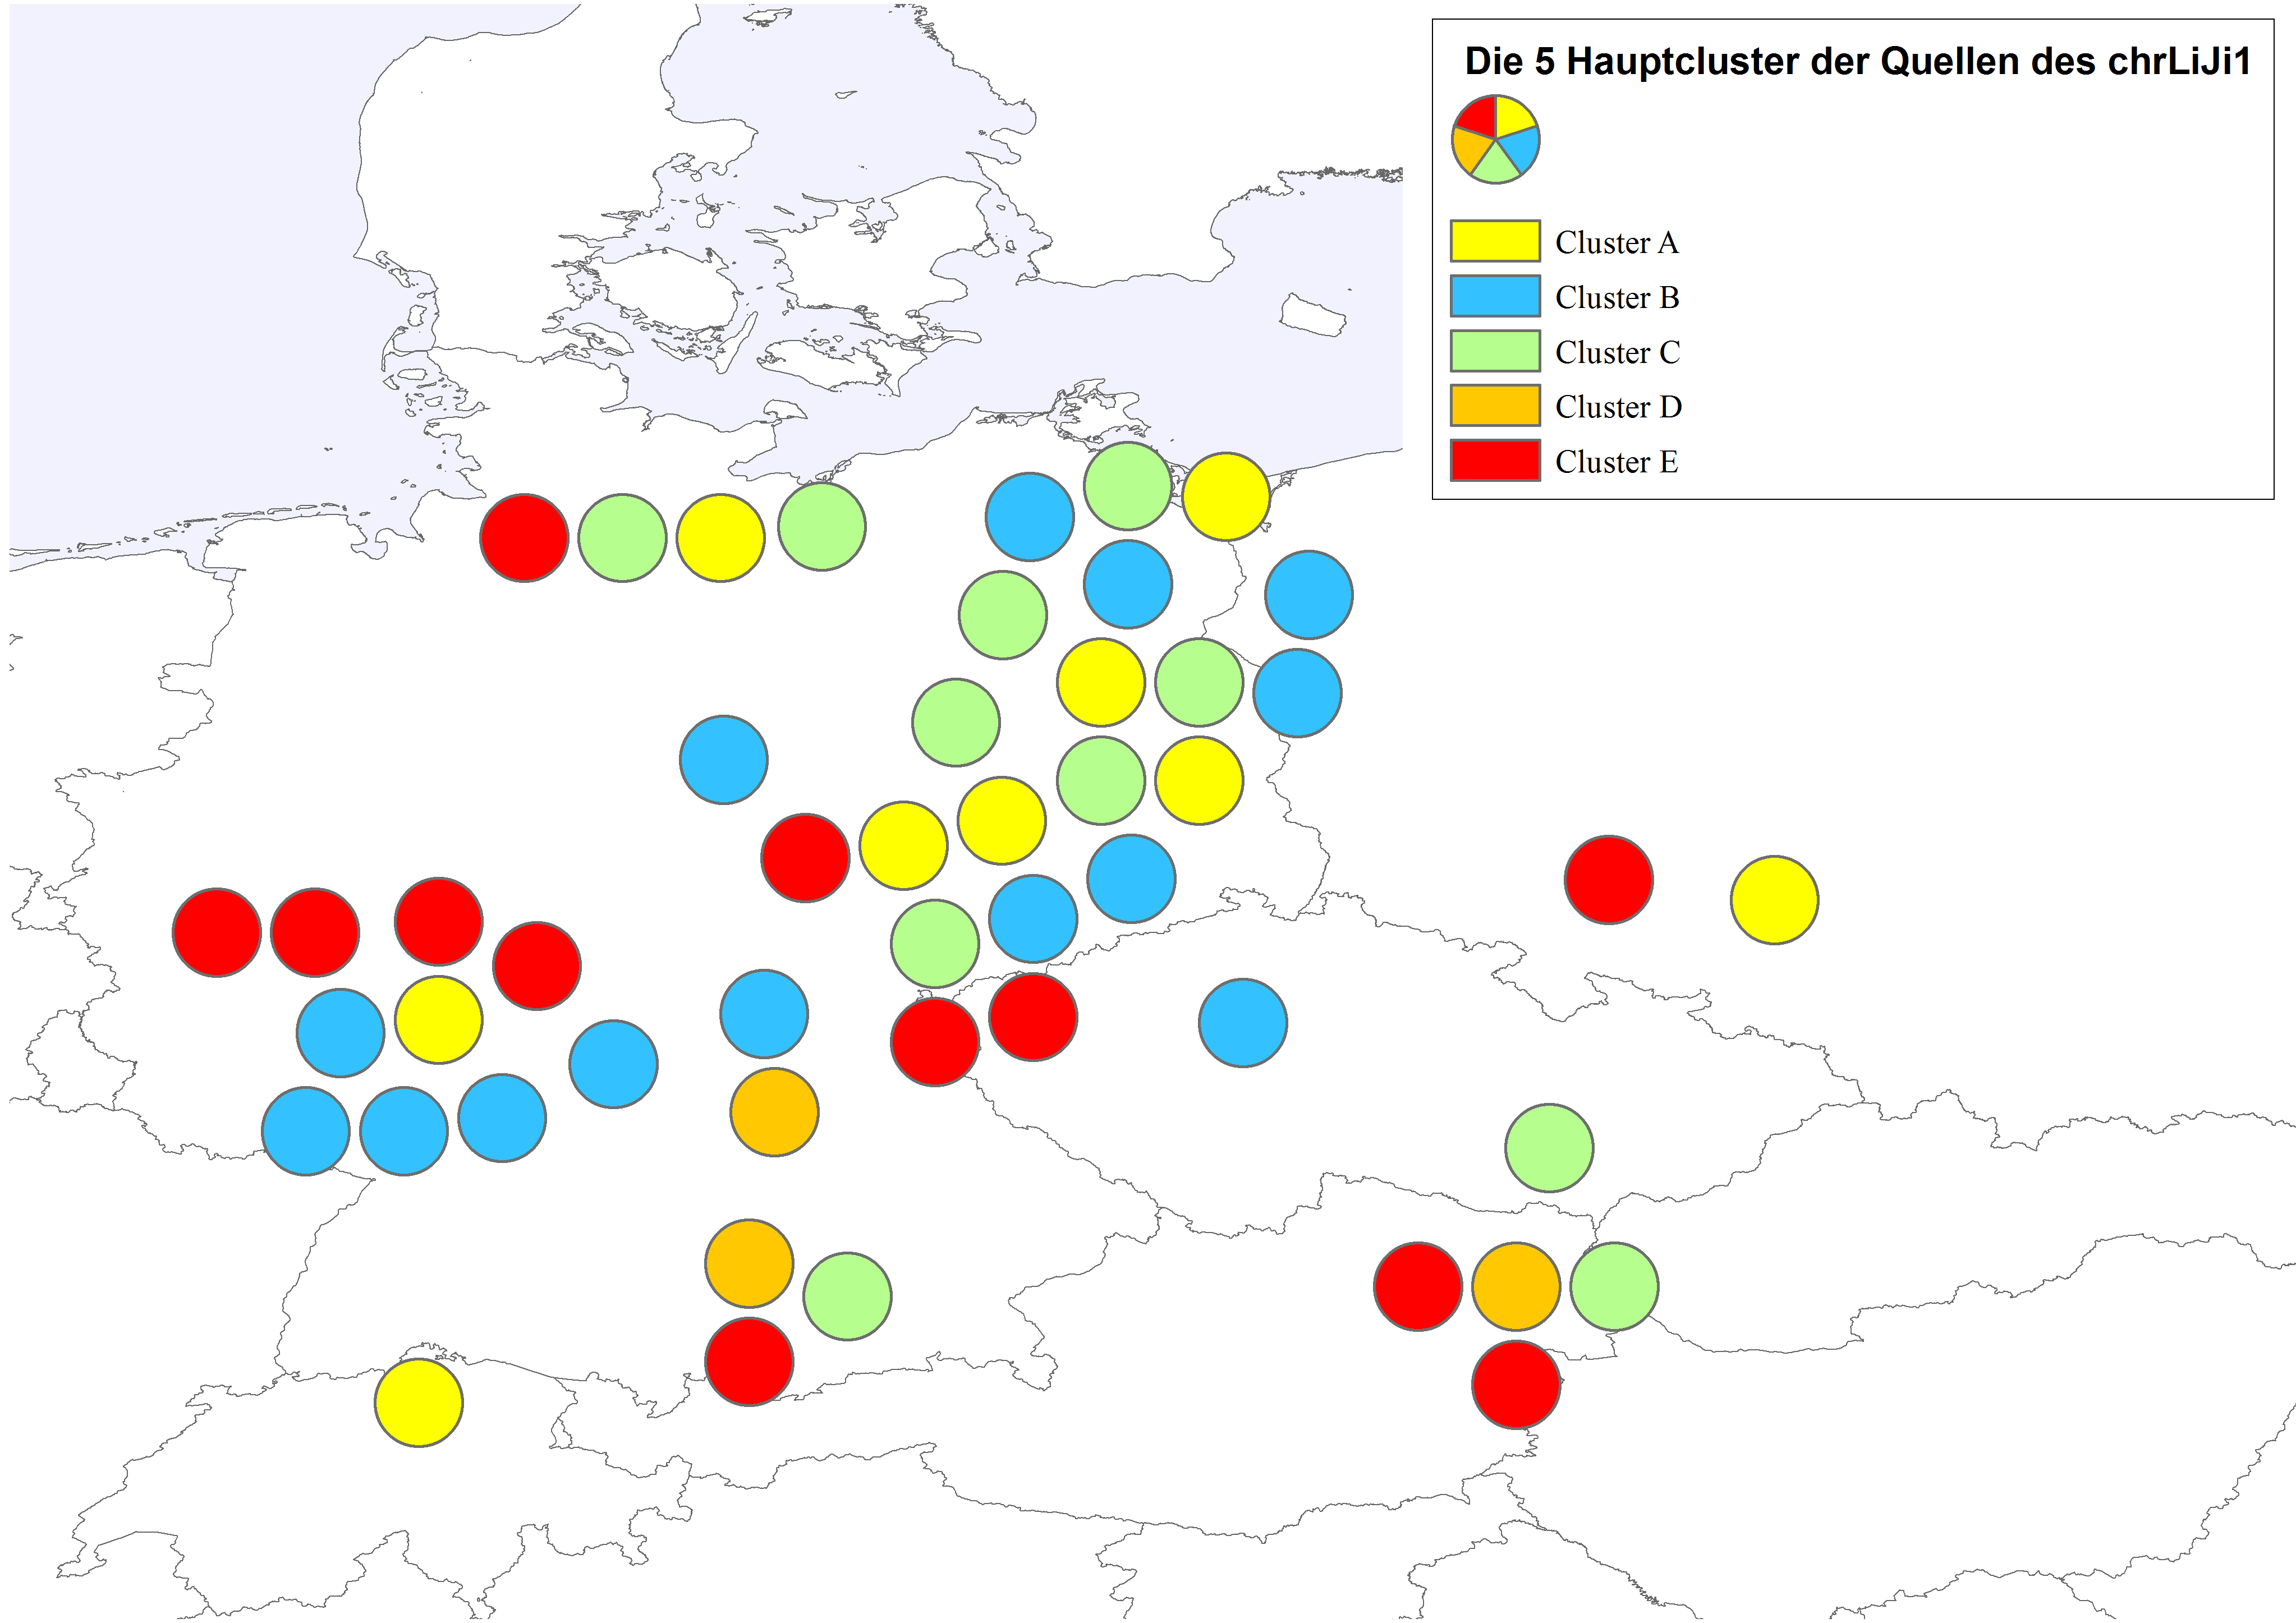
\includegraphics[width=\textwidth]{figures/clusterquellen.png}
		\caption{\label{karteplotcluster} Areale Verteilung der Ward-Clusterung aller \hai{chrLiJi1}-Quellen}
	\end{figure}


%\clearpage

\largerpage
Alles in allem zeigen die Phänomene des \hai{chrLiJi1}, \,%rs ,
 sowie ihre räumliche und zeitliche Strukturen, dass die Autoren sehr wenig \textit{phantasiert}, sondern sehr systematisch gearbeitet haben: Neben Phänomenen, in denen die eigene Dialektalität einfloss, wurden Strukturen des tatsächlich gesprochenen Westjiddischen und z.\,T. des Übergangsjiddischen emuliert. Darüber hinaus spricht die Clusterung der Quellen und deren Phänomene in der Zeit (Abbildung \ref{histoCLUSTERQ}) dafür, dass literarische Traditionen als Katalysator für bestimmte Phänomene gewirkt haben.

	

 \section{Die Rolle des literarischen Dis­kurses am Beispiel Itzig Veitel Stern}\label{IVS}

 Die Marke \quein{Itzig Veitel Stern} ist in der ersten Hälfte des Jahrhunderts weit verbreitet.\footnote{Eine Übersicht bekannter Itzig Veitel Stern Publikationen bietet \citealt{Huggele2016} nebst einer überzeugenden der Aufdeckung des Pseudonyms vom Hauptautor.} Selbst Gustav Freytag reiht sich mit der Namensgebung der Figur \textit{Veitel Itzig} in seinem Roman \qu{Soll und Haben} (\hai{SH} Kluczbork, 1855) in den Dis­kurs ein, obgleich sprachlich keine Übereinstimmungen im \hai{{\LiJi}} Gustav Freytags und denen unter dem Pseudonym Itzig Veitel Stern publizierten Texten vorliegen. Hier beeinflusst der literarische Diskurs das \hai{{\LiJi}} selbst nicht. Anders sieht dies aus bei Nachahmern der  zwischen 1826 und 1938 unter dem Pseudonym Itzig Veitel Stern erschienenen \textit{Originalschriften}. Ein in das \hai{chrLiJi1}-\isi{Korpus} eingegangene Beispiel ist der Pfälzer Autor Christian Heinrich Gilardone (1798–1874)  mit seinen zweibändig erschienenen \qu{Parodiee, Gedichtches unn prousaische Uffsätz'} (\hai{PG} Speyer, 1835), in denen sich der Autor in seinem Vorwort explizit auf Itzig Veitel Stern als sein Vorbild bezieht. Ein anderes Beispiel ist das Exportprodukt eines \textit{originalen} Itzig Veitel Stern Texts (\hai{GP} Nürnberg, 1831) in die Niederlande, wo der Text 1834 im Amsterdamer Verlag H. Moolenijzer, um niederländische Übersetzungen und Ergänzungen erweitert, erschien. Doch nicht in allen Fällen des literarischen Diskurses um Itzig Veitel Stern findet sich \hai{{\LiJi}};oft reicht nur die Verwendung des Namens. Dies ist etwa der Fall im 1848 unter dem Pseudonym \textit{Max Veitel Stern} erschienenen Pamphlet \qu{Die jüdischen Feder=Helden oder Das politisch=literarische Schabesgärtle in Wien}. 

Am Fall des intensiven Diskurs der Figur Itzig Veitel Stern kann exemplarisch nachvollzogen werden, wie groß die Einflüsse der autoreigenen Dialektalität und des literarischen Dis­kurses auf die literarischen Imitationen des Jiddischen sind. Dabei bieten sich besonders der Vergleich dreier Texte an, die als Nachahmungen der Quelle \hai{GP} analysiert werden können. Im Fall von \hai{GP} (Nürnberg, 1831) und \hai{GPndl.} (Amsterdam 1834) liegt sogar ein Paralleltext vor, der den direkten Vergleich ermöglicht. Diese drei im Folgenden näher analysierten Texte sind:

\begin{itemize}
\item [–] Itzig Veitel Stern (Pseud.) \qu{Gedichter, Parabeln unn Schnoukes} (\hai{GP} Nürnberg, 1831)
\item [–] Itzig Veitel Stern (Pseud.) \qu{Gedichten, Parabelen en Sjnoekes of poëtische paarlensnoer voor de kalle} (\hai{GPndl.} Amsterdam 1834)\footnote{Diese Quelle ist nicht Teil des Kernkorpus und wird nur in diesem Kapitel behandelt.}
\item [–] Christian Heinrich Gilardone (1798–1874)\,\qu{Parodiee, Gedichtches unn prou\-saische Uffsätz'} (\hai{PG} Speyer, 1835)
\end{itemize}

Vergleichen wir zunächst einmal die pfälzische Adaption von Itzig Veitel Stern durch Gilardone (\hai{PG}). Wie bereits die Clusteranalyse zur Gruppenbildung der Quellen  gezeigt hat, sind sich die Quellen \hai{GP} und \hai{PG} systematisch sehr ähnlich  (siehe Cluster D in Abbildung \ref{boxplotcluster}, S.\, \pageref{boxplotcluster}). Jedoch unterscheidet sich \hai{PG} rein von der Vielfalt \,%rs Vielfalt
 der Manipulationen vom Vorbild \hai{GP}: Mit 22 Phänomenen ist \hai{PG} deutlich innovativer gegenüber den 14 Phänomenen von \hai{GP} (vgl.\, Abbildung \ref{DiagrammSummePhaen}, S.\, \pageref{DiagrammSummePhaen}). Es ist jedoch interessant, dass \hai{PG} – abgesehen von wenigen lexikalischen Markierungen – dieselben Phänomene aufweist wie \hai{GP}, das \hai{{\LiJi}} seines Vorbildes also um einige weitere Phänomene ergänzt. Neu hinzu kommen bei Gilardone v.\,a.\, morpho-syntaktische Markierungen wie die Verwendung der \isi{Relativpartikel} \textit{wo}, Abfolgevarianz bei zwei- und mehrgliedrigen Verbclustern, \hai{K}-\isi{Diminution} mittels \textit{-che} und die Setzung des Dativs anstelle des Akkusativs nach \isi{Präposition} und bei \isi{Pronomen}. Einige dieser Neuerungen lassen sich auf einen regionalsprachlichen Einfluss des Südrheinfränkischen zurückführen. Doch wären dies auch Formen, die im Dialekt eines ostfränkischen \textit{Itzig Veitel Sterns} zu erwarten wären. So etwa im Fall der \isi{Relativpartikel} \textit{wo}, die im Ostfränkisch wie im  Südrheinfränkischen verbreitet ist (vgl.\, \citealt{Fleischer2005b}, \citeyear*{Fleischer2004d}). 
 Die Unterschiede zwischen beiden Quellen sind also weniger aufschlussreich, vielmehr sind es ihre Gemeinsamkeiten;\, insbesondere jene, die charakteristisch für den Urtext (\hai{GP}) sind und vom Nachahmer übernommen wurden, obwohl sie dem, was wir über westjiddische Varietäten wissen, widersprechen. Ein solches Phänomen ist die Bildung des Diminutiv Singular mittels \textit{-lich}, des Suffixes zur Pluraldiminution im Ost- wie (Süd-)Westjiddischen (vgl.\, Kapitel \ref{dim};ab S.\, \pageref{dim}). Diese Hyperkorrektur findet sich in \hai{GP}  ebenso wie in \hai{PG}. Es ist anzunehmen, dass \hai{PG}  diese Bildung blind von \hai{GP} übernommen hat.\footnote{Dies ist besonders unter dem Umstand interessant, als dass Gilardone das Prinzip der Pluraldiminution mittels \textit{-lich} aus einem nicht unweit seiner Wohnorte Grünstadt u. Speyer liegenden deutschen Dialekt bekannt hätte sein müssen (vgl.\, \hai{WA} Karte Nr. 381).} Für die übrigen Übereinstimmungen zwischen \hai{GP} und \hai{PG}  lässt sich nicht eindeutig differenzieren, ob hier ein Einfluss der Vorlage (\hai{GP}) gegeben ist oder ob sie auf westjiddischen und/oder südrheinfränkischen Formen basieren. Der Einfluss des populären Vorbilds (\hai{GP}) auf den pfälzischen Nachahmer (\hai{PG}) darf aber nicht unterschätzt werden. %Bezeichnend ist die Feststellung, dass \hai{PG}  dieselben Manipulationen zeigt wie \hai{GP} (Nürnberg, 1831) und dessen Repertoire nur um wenige Phänomene ergänzt.

Während die Bearbeitung des Itzig Veitel Stern-Stoffes in \hai{PG}  noch sehr frei ist, liegt uns mit \hai{GPndl.} (Amsterdam 1834) eine direkte niederländische Edition des Urtexts (\hai{GP}) vor. Die Frage ist hier: Wurde der Text \hai{GP} lediglich an die niederländische \isi{Orthographie} angepasst oder finden sich in \hai{GPndl.} auch Formen, die vom \hai{{\SWJ}} des Urtexts abweichen und Strukturen des niederländischen \hai{{\NWJ}} repräsentieren. In Tabelle \ref{paralelltextIVS} sind Urtext und niederländische Edition in einem Ausschnitt gegenübergestellt.\footnote{Die {\ndl} Übersetzung der Strophe (\hai{GPndl.} Amsterdam 1834:\,2) wird hier nicht näher diskutiert, da das \hai{{\LiJi}} der beiden Texte relevant ist.} Neben Unterschieden in der \isi{Interpunktion} fällt besonders die inhaltliche Abweichung in Zeile 2 auf. Wahrscheinlich war hier der Ausdruck \textit{Reisen machen} dem niederländischen Bearbeiter nicht geläufig. Die an dieser Stelle neue zweite Zeile zeigt immerhin, dass der Bearbeiter ein westjiddisches Grundprinzip erkannt hat und anwenden kann: die Monophthongierung von \hai{V24} ({\mhd} \textit{ei}) in \textit{Stahn} \sem{Stein}.\footnote{Möglich ist jedoch auch, dass nicht \hai{GP} die Vorlage für \hai{GPndl.} war, sondern eine andere Ausgabe, in der Zeile 2 wie in \hai{GPndl.} lautet.} Sprachlich interessant an der niederländischen Edition \textit{Itzig Veitel Sterns} ist die Angleichung der \isi{Orthographie}. So bleibt etwa <eu> für /ɔʏ̯/ erhalten, ein Diphthong, den es im Niederländischen nicht gibt ({\ndl} <ui> /œʏ̯/), für /u(\textlengthmark)/ wird aber das niederländische komplexe Graphem <oe> anstelle der deutschen Vorlage <u> gesetzt, um eine Verwechslung mit der niederländischen Entsprechung für <u> als /ø/, /y\textlengthmark/ zu vermeiden. Für den gerundeten Vorderzungenvokal /y/ bleibt das Graphem <ü> der Vorlage erhalten (\textit{Jüden} \sem{Juden} {\ndl} \textit{Joden}). Es wurde also weitestgehend versucht, eine deutsche \isi{Orthographie} beizubehalten und gleichzeitig Interferenzen zum niederländischen System zu vermeiden.
 
 %%%hier ausschnitt paralelltext

	\begin{table}
 \fittable{
\small
	\begin{tabular}{rll}
\lsptoprule
& \textbf{Urtext} (\hai{GP} Nürnberg, 1831:\,5)  & \textbf{{\ndl} Edition} (\hai{GPndl.} Amsterdam 1834:\,1) 	 \\ \midrule % horizontale Trennlinie
& &\\
\small{1} & \textit{Drey Wörtlich nenn ich Euch, se senn schwer,}	&\textit{Drey Wörtlich nenn ich Euch, se sen schwer} \\
&\textit{Unn machen gewaltige Reisen,} & \textit{Noch schwerer wie Stahn, oen wie Eisen,}\\
&\textit{Se stammen von unnere Leute her,} & \textit{Sie stammen von oensere Leute her,}\\
&\textit{Mer kenne ousn Talmud beweisen;} & \textit{Merr kenn's aus'n Talmud beweisen;}\\
\small{5} &\textit{Diem Jüden is aller Wert geroubt,}&\textit{\qu{Dem Jüden is aller Wert beraubt,}}\\
&\textit{Wenn er nimmer on die drey Wörtlich gloubt.}&\textit{\qu{Wenn er nimmer an die drey Wörtlich glaubt.}}\\ 
\\
\end{tabular} 
}
\small
\begin{tabularx}{\textwidth}{X}
\sem{Drei Wörtchen nenne ich euch, sie sind schwer / Und haben einen großen Weg hinter sich [\hai{GPndl.}: Noch schwerer wie Stein und wie Eisen] / Sie stammen von unseren Leuten / Man kann es aus dem Talmud beweisen / Den Juden ist aller Wert geraubt / Wenn er nicht mehr an die drei Wörtchen glaubt.}\\
\lspbottomrule
\end{tabularx}
 

\caption{\label{paralelltextIVS} Ausschnitt der Paralelltexte \hai{GP} und \hai{GPndl.}} 
\end{table}

 
Einziger Hinweis auf einen direkten Einfluss des niederländischen \hai{{\NWJ}} lässt sich in der Graphie für \hai{V42} ({\mhd} \textit{ô}) finden. Während \hai{GP} hier den für das \hai{{\SWJ}} und Teile des \hai{{\ZWJ}} üblichen Diphthong /ou/ als <ou> setzt (\textit{geroubt} \sem{geraubt}, \textit{gloubt} \sem{glaubt};vgl.\, Kapitel \ref{phonV42}, ab S.\, \pageref{phonV42}), verwendet \hai{GPndl.} an dieser Position systematisch das Graphem <au> (\textit{beraubt} {\ndl} \textit{beroofd}, \textit{glaubt} {\ndl} \textit{gelooft}). Im Niederländischen stehen die Grapheme <au> und <ou> gleichermaßen für den Diphthong /ʌu̯/ (der zwischen /\textopeno \textsubarch{u}/ und /a\textsubarch{u}/ liegt). Die Motivation hinter dem Wechsel vom <ou> der Vorlage zu <au> in \hai{GPndl.} ist nicht erkennbar;\, denkbar wäre, dass der niederländische Bearbeiter mit der <au>-Graphie \quein{hochdeutscher} wirken wollte. Nach Beem (\citeyear[127]{Beem1954}) ist im niederländischen \hai{{\NWJ}} \hai{V42} ({\mhd} \textit{ô}) noch die ältere Form /\textopeno \textsubarch{u}/ anzutreffen und nicht etwa /a\textsubarch{u}/. Doch Beems Daten beruhen größtenteils auf mitteljiddischen Quellen, deren Graphem-Phonem-Relation generell problematisch ist. In den Karten Guggenheim-Grünbergs (\citeyear{GuggenheimGruenberg1973}) zur Situation im 20. Jahrhundert zeigt sich ein deutlich uneinheitlicheres Bild im niederländischen \ili{Westjiddisch}: besonders bei Hebraismen ist /o\textlengthmark/ bereits als /a\textsubarch{u}/ bezeugt (\citealt[Karten 13 u. 20]{GuggenheimGruenberg1973}), während in Germanismen noch /\textopeno \textsubarch{u}/ weitestgehend erhalten blieb (\citealt[Karte 16]{GuggenheimGruenberg1973}).\footnote{Doch hier muss berücksichtigt werden, dass Beem (\citeyear[127]{Beem1954}) eine Quelle des {\ndl} \hai{{\NWJ}} für Guggenheim-Grünberg (\citeyear{GuggenheimGruenberg1973}) ist.} Für das \hai{{\NWJ}} Deutschlands ist \hai{V42} als bislang ausschließlich /a\textsubarch{u}/ belegt (vgl.\, Beispiele in \ref{bsp42WJ}, S.\, \pageref{bsp42WJ}). Alles in allem lässt die vom Urtext abweichende Schreibung <au> für \hai{V42} ({\mhd} \textit{ô}) in \hai{GPndl.} die Vermutung zu, dass der Diphthong die regionale Aussprache des Dipthongs näher an /a\textsubarch{u}/ als an /\textopeno \textsubarch{u}/ lag.

Der Vergleich der zwei Itzig Veitel Stern-Bearbeitungen mit der Vorlage zeigt, dass der Einfluss des literarischen Diskurses eine wichtige Rolle im \hai{{\LiJi}} spielt und nicht unterschätzt werden darf. Allerdings ist er in den wenigsten Fällen so deutlich nachzuvollziehen wie im Fall der Adaptionen der Itzig Veitel Stern-Mode. 


\section{Vergleich der Verteilung der Phänomene im \hai{chrLiJi1} und \hai{jüdLiJi1}}\label{phaenomene}% und \hai{LiJi2}
%\noindent
Nun gilt es die erhobenen Daten der Beiden Korpora \hai{jüdLiJi1} und \hai{chrLiJi1} quantitativ zu bündeln und miteinander zu vergleichen. Die Tabellen (S.\, \pageref{appendixphaenall} und S.\, \pageref{appendixphaenalljuedliji}) im Appendix führen die nachfolgenden quantitativen Ergebnisse relevanten Phänomene und ihr Auftreten in den Subkorpora auf. 

Eine Quelle des \hai{jüdLiJi1} zeigt durchschnittlich 23,5 Phänomene bei einer Standardabweichung von $\sigma$\,5,5 Phänomenen. Die letzte Ausgabe der \qu{Gedichte und Scherze in jüdischer Mundart} (\hai{GuS23}) verwendet mit 29 von 58 Phänomenen die meisten unterschiedlichen Strategien. Die zwei Quellen mit den geringsten Phänomenwerten sind \hai{GuS15} (16 Phänomene) und \hai{PDebrecen} (12 Phänomene). Es ist kein signifikanter quantitativer Unterschied zwischen den Quellen der \qu{Gedichte und Scherze} und den Pamphleten zu erkennen. Die häufigsten im \hai{jüdLiJi1} auftretenden Phänomene sind \hai{{\NP}}-Extrapositionen (in allen zehn Quellen gegeben), gefolgt von \hai{{\PP}}-Extrapositionen, \hai{{\VR}}, \textit{a}-Verdumpfungen und der westjiddischen Monophthongierung von \hai{V24} (die in jeweils neun Quellen auftreten).
Im Vergleich zu den durchschnittlich 13 Phänomenen des \hai{chrLiJi1} (Standardabweichung 7) unterscheiden sich die Texte des \hai{jüdLiJi1} besonders deutlich. 
	
    Das Ergebnis der Clusteranalyse zur Phänomenverteilung (58 Phänomene) der Korpora (\hai{chrLiJi1} und \hai{jüdLiJi1} zusammen 61 Quellen) in Abbildung \ref{dreikorporaplotcluster} zeigt eine nicht zufällige Verteilung. Quellen des \hai{jüdLiJi} (unterstrichen in Abbildung \ref{dreikorporaplotcluster}) finden sich nahezu ausschließlich in einem Hauptcluster gesammelt. Nur eine Quelle (\hai{PDebreczen}) fällt deutlich aus dem Rahmen der \hai{jüdLiJi1} Quellen. Im \,%rs im
    Hauptcluster, \,%rs ,
    in dem sich die Quellen jüdischer Autoren sammeln, sind elf Quellen des \hai{chrLiJi1} zu finden, was 21\% des Gesamtsamples zum \hai{chrLiJi1} ausmacht. 
Die gemeinsame Clusterung eines Großteils der \hai{jüdLiJi1}-Quellen in einem Hauptcluster lässt sich besonders über die geographische Lage im Berliner Raum erklären;\, sie könnte aber auch ein Hinweis darauf sein, dass sich die Sprache jüdischer Autoren generell von der nicht-jüdischer Autoren unterscheidet. Um dies letzten Endes klären zu können, ist eine Analyse weiterer, nicht aus dem Nordosten stammender Quellen jüdischer Autoren notwendig. Alles in allem weisen die untersuchten Quellen zum \hai{jüdLiJi1} deutlich mehr an das Ostjiddische anlehnende Strukturen auf, was mit Blick auf die räumliche Verteilung dieser Quellen im Nordosten des Untersuchungsgebiets erklärbar ist. Aber auch der urbane Raum in dem diese Quellen ihren Sitz-im-Leben haben, mag die Verwendung ostjiddischer Strukturen begünstigt haben.  Interessant ist hier auch die Verortung der elf \hai{chrLiJi1} Quellen, dich in diesem Hauptcluster zur Folge dem \hai{jüdLiJi1} strukturell \,%rs strukturell
besonders nahe stehen. Diese Quellen stammen überwiegend aus Großstädten\footnote{Neben der eher ländlichen Quelle \hai{TH} (Merseburg, 1820) stammen diese Quellen aus Berlin (\hai{MV}, \hai{SS}), Frankfurt a.\,M. (\hai{VD}, \hai{PA}), Hamburg (\hai{AB}, \hai{JP}), Leipzig (\hai{FE}), Zürich (\hai{AK}) und München (\hai{SV}). \\
Desweiteren ist zu erwähnen, dass die Quelle \hai{VD} einen aus dem Judentum konvertierten Autor als Mitautor nennt: Maximilian Leopold Langenschwarz (geb. 1808 in Rödelheim als Meyer Hoffmann und 1830 zum Protestantismus konvertiert). Mit Blick auf das Ergebnis \,%rs Ergebnis
der Clusteranalyse in Abbildung \ref{dreikorporaplotcluster} lässt sich die Vermutung äußern, dass die Quelle \hai{VD} ggf. eher den Quelltyp \hai{jüdLiJi1} vertritt, als dass sie \hai{chrLiJi1} repräsentiert;\, den Hinweis auf die Hintergründe zu Langenschwarz' Herkunft verdanke ich Marco Huggele (Esslingen).}, \,%rs ,
 in denen ein potenzieller ostjiddischer Einfluss besonders wahrscheinlich \,%rs wahrscheinlich
ist.\\ 
Es ist bezeichnend, dass die fünf Hefte der \hai{GuS} zwar im selben Hauptcluster zu finden sind, allerdings nur die Hefte \hai{GuS5} und \hai{GuS15} gemeinsam ein Subcluster bilden. Dies spräche dafür, im Fall der beiden Texte einen gemeinsamen Autor anzunehmen bzw. spräche
das Resultat der Clusteranalyse im Umkehrschluss dafür, für die unterschiedlichen Hefte der \hai{GuS} auch unterschiedliche Autoren anzunehmen. Diese Hypothese müsste selbstverständlich durch philologische Beobachtungen überprüft werden. 

\begin{figure}
\centering
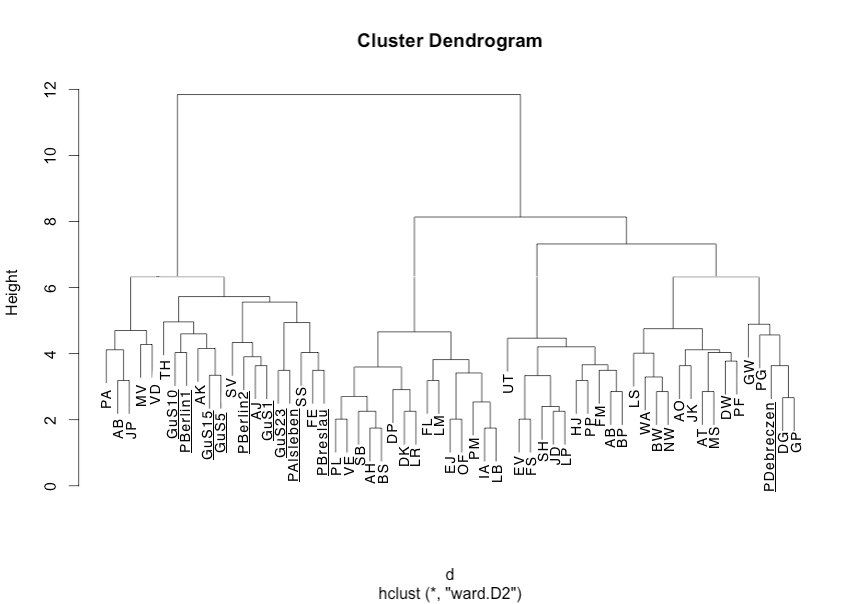
\includegraphics[width=\textwidth]{figures/ClusterneuOHNEliji2.jpg}
		\caption{\label{dreikorporaplotcluster} Ward-Clusterung der Quellen der zwei Korpora \hai{chrLiJi1} und \hai{jüdLiJi1}}
	\end{figure}

%\newpage
%\clearpage

	
\noindent Um zu testen, wie nahe die Imitationen ihren Zielsprachen kommen, wurde ein Datenset zu den entsprechenden Phänomenen für Proto-\ili{Westjiddisch} und Proto-\ili{Ostjiddisch} aus den Ergebnissen der Einzelanalysen erstellt. Die Clusteranalyse zu allen Korpustexten und diesen Proto-Varietäten in Abbildung \ref{WJOJcluster} \,%rs ist streichen
 hat zwei Seiten: Zum einen ist keine der literaturjiddischen Quellen mit den gesprochenen Sprachen identisch bzw. die Clusterung zeigt \,%rs , streichen
 sogar, dass sich \hai{{\WJ}} und \hai{{\OJ}} deutlich näher sind als die literarischen Imitationen. Doch das heißt nicht, dass  die literaturjiddischen Quellen nicht korrekte jiddische Formen produzieren, sondern lediglich, dass keine Quelle in der Gesamtheit und Verteilung der Phänomene den natürlichen Sprachen entspricht, sondern eben nur einzelne Elemente dieser Sprache in ein anderes System emuliert werden. In gewisser Hinsicht bestätigt das Bild in Abbildung \ref{WJOJcluster} sogar die Idee der emulierenden Sprachimitation: Ein sprachliches System wird nicht vollumfänglich nachgeahmt, sondern nur einzelne Elemente, die genug Zeichenwert  besitzen, um auf das imitierte System zu verweisen. Und dies ist die zweite Seite. Wir sehen mit der Clusterung, welche Quellen besonders nah an die natürlichen Varietäten heranreichen: Dies sind die Quellen des \hai{jüdLiJi1} (mit Ausnahme von \hai{PDebreczen}) und die elf Quellen des \hai{chrLiJi1}, die mit ihnen clustern (s.o.). Mit diesem Ergebnis \,%rs Ergebnis
 lässt sich behaupten, dass die jüdischen Autoren insgesamt genauer die Sprachrealität wiedergeben als die nicht-jüdischen. Dies ließe sich auf noch (in Resten) vorhandene muttersprachliche Kompetenz und/oder mit einem engeren Kontakt zu aktiven Sprechern des Jiddischen erklären. 	
 

	\begin{figure}
%\centering
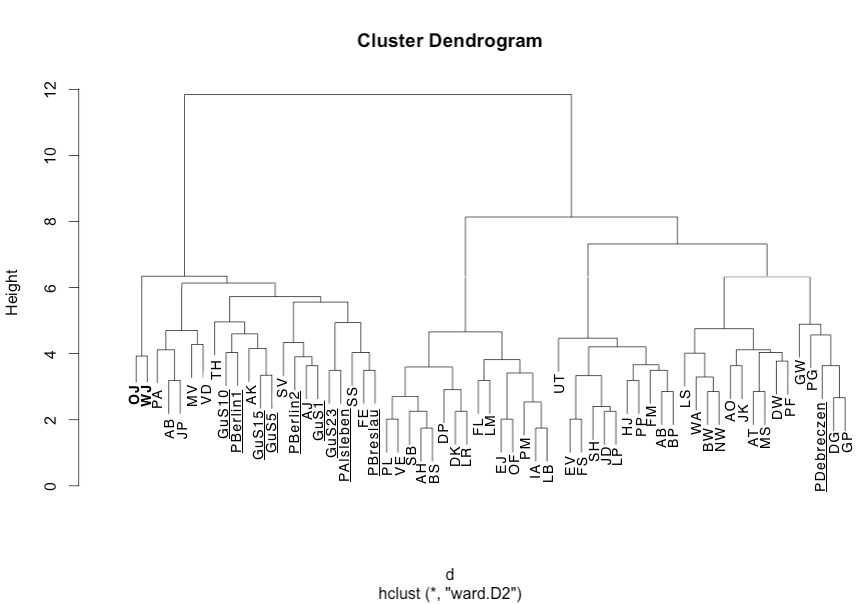
\includegraphics[width=\textwidth]{figures/ClusterneuOJWJ.jpg}
		\caption{\label{WJOJcluster} Ward-Clusterung aller zwei Korpora zzgl. \hai{{\WJ}} und \hai{{\OJ}} }
	\end{figure}


